%% TestVDB — FSE 2027 submission (rewritten from scratch, 2026-09-05)
%% Confirmed numbers ONLY: RQ1 = 81 submitted / 51 confirmed / 23 fixed / 30 FP
%% (ledger: data/phase1_issue_classification.xlsx, 9149 disproved & meilisearch excluded).
%% RQ2 clean pool (cognition stripped + re-judge, then candidate-anchored cognition
%% entries removed + 7-case re-judge both backbones, 2026-09-13):
%% core 0.157/0.967, full 0.765/0.700, flat 0.588/0.867, source-only 0.706/0.733,
%% source-only-Qwen 0.725/0.700.
%% Pack audit: 134 constraint-page pairs, 43.3% unsupported (58 DROP), 2 over-strong.
%% HUMAN_REVIEW counts as CONFIRMED in the study aggregation (disclosed in 4.3).
%% Replication archive live at the anonymized URL in Data Availability.
%% FSE 2027 format: acmsmall single-column, 18 pages text+figures + 4 pages refs.
%% Deadline: 2026-10-02 AoE. Data Availability section required after Conclusion.
\documentclass[acmsmall,screen,review,anonymous]{acmart}

\usepackage{tikz}
\usetikzlibrary{positioning, arrows.meta}
\emergencystretch=2em
\settopmatter{printacmref=false}
\settopmatter{printfolios=false}
\newcommand{\system}{TestVDB}

\begin{document}

\title{Detecting Logic Bugs in Vector Database Management Systems via LLM-Derived Behavioral Specifications}

\begin{abstract}
Vector Database Management Systems (VDBMSs) store the embeddings that retrieval-augmented LLM applications depend on, yet most of their bugs are logical bugs that produce no crash and thus escape crash-oracle fuzzers such as VDBFuzz. We target \emph{documentation-implementation bugs}: cases where a VDBMS silently accepts an input or produces a behavior that violates its API documentation---constraints no structured source such as an OpenAPI schema declares---such as accepting \texttt{nprobe=0} when the documentation declares the range as $[1, 16384]$. Because the documented boundary is natural-language prose, no deterministic-oracle family we analyze derives its expectation from that behavioral prose---crash signals, reference implementations, output relations, and schemas all anchor elsewhere, and the constraint-inference line that does read prose stops at parameter-level declarations---leaving an LLM as the practical oracle, and importing its false-positive problem.

We instantiate \system{}, a four-stage pipeline whose confirmation stage cross-examines a five-section evidence chain from four perspectives---contract, physical constraints, behavioral elegance, and maintainer cognition---with the implementation source as the falsification anchor---which the controls price: withholding the source clone raises recall to 0.941 and cuts suppression to 0.467, so on the summary metrics it is the cheaper configuration, and the source is what refuses candidates rather than what finds them. Across Milvus, Qdrant, and Weaviate, in an operational human--machine deployment with author-side screening and submission, maintainers confirmed 51 of 81 adjudicated submissions as real bugs and fixed 23 via merged PRs. The ledger is the sum of sixteen per-version mining campaigns (February--August 2026) and predates the run reported here, which contributed none of the 81; the automated stage's own measured behavior is reported separately below.

An audit of the frozen evidence packages that fed our confirmation stage found 43.3\% of their cited (constraint, page) pairs unsupported by the referenced documentation pages; after rebuilding every package against version-pinned documentation and re-adjudicating the full pool three times under the deployment protocol, the contract-only core suppresses 96.7\% of the 30 adjudicated false positives but recalls 0.157 of the 51 confirmed bugs, while the structured full stage reaches 0.765 recall at 0.700 suppression under the deployment's counting convention---against 0.588 for a flat single-prompt judge reading the same packs and sources. The deployment's own reading is that counting convention, since the deployment reports what the protocol routes; the other two readings we report are sensitivities around it. Forced verdicts are a conservative floor, where the two judges collapse to indistinguishable recall (0.529 vs.\ 0.490). A hand-adjudicated review of the routed queue---a stricter standard than the deployment applies, and author-executed---lands between them at 0.647 recall and 0.917 precision, with an independent adjudicator working from the same materials and the full deployed rules reaching 0.588. Routing, not forced accuracy, is where the gain lies---a flat judge bound to the same aggregation rule matches the full stage's recall without its four perspectives, whose own increment is not established here---and on metrics that price a confirmed false positive against a confirmed true positive the full stage still leads on both backbones (30 vs.\ 26 net on the primary family, 25 vs.\ 22 on the second).

That separation survives Holm correction on the confirmed-set unit against the shipped flat dispatch---the statistic the deployment resolves, though five of its fourteen net cases are additional false-positive confirmations, and the recall-only comparison does not survive (Holm-adjusted 0.090)---but against the same arm with its dispatch repaired it is 48 against 39, raw $p{=}0.049$, which does not survive correction; and it is measured on one model family; a three-run re-run of the pair on a second family does not separate ($p{=}0.58$). A bidirectional probe against VDBFuzz on Qdrant shows complementary reach: run to natural completion on the instance where our silent-accept defects are live, its full released template set reaches none of them, while a hand-guided probe built on \system{}'s boundary reasoning reaches VDBFuzz's crash-class integer overflow on v1.4.0.
\end{abstract}

\maketitle

\section{Introduction}
\label{sec:intro}

Vector Database Management Systems (VDBMSs) such as Milvus, Qdrant, and Weaviate have become core infrastructure for retrieval-augmented LLM applications: they store the embeddings and serve the similarity queries from which the model's context is assembled. When a VDBMS query is buggy, the wrong context reaches the model---a disabled filter returns all matches, a zero-length vector corrupts an index, a dropped partition hides expected data---and the error propagates into generated text with no crash and no error code to log.

Empirical studies show that this failure shape is the norm, not the exception: most VDBMS bugs are functional failures that keep the service up while silently returning wrong results~\cite{bugstudy25,roadmap25}. The one dedicated VDBMS fuzzer, crash-oracle by design (its own reported results are 13 crash vulnerabilities plus six runtime exceptions), is VDBFuzz~\cite{vdbfuzz26}; it targets the complementary minority---crash signals from mutated API requests---so the silent majority is out of its reach by construction. Our own ledger agrees: one of the 51 maintainer-confirmed bugs (Section~\ref{subsec:rq1}) produces a crash or panic---Qdrant \#9045, where a silently accepted zero-length vector panics a later search (Table~\ref{tab:bug-patterns}, the \textsc{Other} row).

We target a prevalent subset of this silent majority: \emph{documentation-implementation bugs}, where a VDBMS silently accepts an input or produces a behavior that violates its API documentation. A canonical instance of the class: Milvus documents \texttt{nprobe} as an integer in $[1, 16384]$, yet the search API accepts \texttt{nprobe=0} with HTTP 200 and returns results (issue~\#49823). Detecting such bugs requires an expectation derived from the documentation itself, and here every deterministic-oracle family we analyzed falls structurally short (Table~\ref{tab:exclusion}, whose rows 2--7 are argued from each family's anchoring mechanism rather than exercised): each anchors its expectation in a crash signal, another implementation, an output--output relation, a machine-checkable property, or a structured spec---none in the prose itself. One further family needs separating out because it is a component of our own stage: a catalogue of objective constraint classes (perspective~B, Section~\ref{subsec:confirmation}) is deterministic and reads no documentation, and it drives 16 of the full stage's 39 confirmations. It is not an independent oracle, because it supplies only a falsifier for what a system must not do---a limit parameter accepting zero, a closed enum admitting a stray value---and no expectation about which behaviors to exercise; the probes that reach those cases still come from constraints read out of the prose, and the catalogue fires only on an observation that already exists. It nevertheless belongs in the table, as row 7 of Table~\ref{tab:exclusion}, because omitting it would overstate the residual: it reaches part of the class with no prose at all, so what the prose is needed for is narrower than the other rows alone imply. Reading the prose is a semantic-interpretation step that only an LLM currently performs at scale---leaving an LLM-derived oracle as the practical option.

Putting an LLM in the oracle role imports a false-positive problem. The same model family that misreads an ambiguous sentence into an over-strong constraint later judges whether the observed behavior violates it; hallucination at extraction, self-preference at judgment, and run-to-run inconsistency all push candidates toward confirmation. A multi-perspective panel does not fix this: every judge reads the same ambiguous documentation, so the ambiguity is shared, not broken.

\system{} (Section~\ref{sec:approach}) answers with a four-stage pipeline in which the falsification is grounded outside the LLM: documentation is distilled into source-verified specifications, attack agents turn them into executable probes under pre-bound strategies, a sandbox runs every probe against a Docker-pinned version while logging raw HTTP traffic, and a bug-confirmation stage splits evidence assembly from cross-examination. Every verdict carries a source-grounding section, and the source---independent of the documentation the specification was read from---is the falsifier that breaks the self-referential loop: by-design refutations require verbatim in-source intent evidence, and the absence of a validation the contract predicts is located in the code. Contract and objective-constraint confirmations do not need source evidence, which is why the pack-only core still confirms eight cases.

Across Milvus, Qdrant, and Weaviate, maintainers confirmed 51 of 81 adjudicated submissions as real bugs and fixed 23 via merged PRs (Section~\ref{subsec:rq1}); that ledger carries author-side screening and the submission decision, so it measures the human--machine pipeline rather than the automated stage alone. Because the frozen evidence packages that fed our confirmation stage turned out to be the weakest link---an audit found 43.3\% of their cited (constraint, page) pairs unsupported by the pages they cite---we rebuilt every package against version-pinned documentation and re-adjudicated the full pool three times per configuration under the deployment protocol (Section~\ref{subsec:rq2}). The contract core suppresses 96.7\% of the 30 adjudicated false positives but recalls 0.157 of the 51 true bugs; the full structured stage reaches 0.765 recall at 0.700 suppression, and a flat single-prompt judge reading the same packs and sources reaches only 0.588---the advantage survives Holm correction ($p{=}0.0052$), and 19.8\% of the full stage's verdicts route to an explicit human-review channel rather than being forced. The decomposition attributes the separation to that routing channel, and the two are separable: adding the aggregation rule to the flat judge, with no perspective vocabulary and no evidence-chain sections, recovers the full stage's recall exactly (0.765; indistinguishable, $p{=}0.61$), so the four-perspective organization's increment is not established on this pool. Under forced verdicts alone the two judges are indistinguishable---and the comparison is a single-backbone measurement: the second model family's source-only arm separates from the flat judge after correction in a cross-family pairing, but the full-vs-flat pair re-run three times on that family does not separate ($p{=}0.58$) (Section~\ref{subsec:rq2}). A bidirectional probe against VDBFuzz (Section~\ref{subsec:rq3}) shows the oracles are complementary: run to natural completion against the instance where our silent-accept defects are live, VDBFuzz's released template set---its template-mutation stage, not the sequence-mutation stage its paper also describes---reaches none of them, while a hand-guided probe built on \system{}'s boundary reasoning reaches VDBFuzz's crash-class integer overflow on v1.4.0.

This paper makes three contributions:
\begin{itemize}
  \item \textbf{Problem and oracle analysis.} We formalize documentation-implementation consistency testing for VDBMSs and give a structural account of why every deterministic-oracle candidate misses it (Table~\ref{tab:exclusion}), delimiting where an LLM-derived oracle is forced.
  \item \textbf{\system{} pipeline.} A four-stage, multi-agent pipeline whose confirmation stage grounds every verdict in evidence sources outside the LLM---above all the implementation source, the only channel that may refute---to break the extraction-judgment self-reference. The confirmation stage's routing aggregation is the measured mechanism on the primary backbone, not a law of the protocol: reading the same packs and sources the full stage recalls 0.765 where a flat single-prompt judge reaches 0.588, a gap carried by the routing channel rather than by forced-verdict accuracy---and the two are separable, since adding the aggregation rule to the flat judge, with no perspective vocabulary and no evidence-chain sections, recovers the full stage's recall exactly (0.765; indistinguishable, $p{=}0.61$), so the four-perspective organization's increment is not established on this pool; the paired difference in \emph{confirmed sets} is 48 vs.\ 34 (exact McNemar $p{=}0.0013$, Holm-corrected $0.0052$), but five of its fourteen net cases are additional false-positive confirmations and the recall-only comparison does not survive correction (raw $p{=}0.0225$, Holm-adjusted 0.090), and a three-run re-run of this pair on a second family does not separate ($p{=}0.58$); its verdicts admit three readings, reported side by side (forced verdicts 0.529, joint judge-plus-human 0.647, counting convention 0.765); and the decomposition attributes the convention-based separation to its explicit human-review routing, which converts unresolvable cases into adjudicable ones instead of forced closures (Section~\ref{subsec:rq2}).
  \item \textbf{Empirical evidence.} 51 maintainer-confirmed real bugs (23 fixed) across three production VDBMSs; a controlled nine-arm evaluation over audited and rebuilt frozen packages that reports both sides of the tradeoff (0.765 recall at 0.700 suppression for the full stage; the contract core at 0.157/0.967) plus independent source-only and flat-judge arms, the two component controls that locate the separation on the routing rule, and the source-withheld control that prices the falsification anchor; and a bidirectional complementarity probe against the crash-oracle baseline.
\end{itemize}

\section{Background and Motivation}
\label{sec:prelim}

\subsection{Bug Distribution and the Non-Crashing Majority}
\label{subsec:bugs}

Empirical studies of VDBMS defects converge on one structural fact: most VDBMS bugs do not crash. The systematic bug study~\cite{bugstudy25} attributes the dominant share to functional failures---the system stays up but silently returns wrong results---while crash-signal bugs are a minority class~\cite{bugstudy25,roadmap25}. The dedicated fuzzer VDBFuzz~\cite{vdbfuzz26} reaches exactly that minority: its oracle fires on crash signals from template-based input mutation. The testing roadmap~\cite{roadmap25} names oracle definition as the key open challenge for precisely this residual.

\subsection{Documentation-Implementation Inconsistency}
\label{subsec:consistency}

We target a prevalent subset of the non-crashing majority: \emph{documentation-implementation inconsistency} (Section~\ref{sec:intro}). We separate consistency from \emph{correctness}: consistency asks whether the system's observable behavior---what it accepts, what it errors on, what it returns, and how its state evolves---matches what its API documentation prescribes; correctness asks whether a returned result is mathematically right, such as ANN recall or ranking. \system{} targets consistency; result correctness of vector search remains open and is not our claim~\cite{roadmap25}. The reverse shape also arises: an operation the documentation prescribes as atomic or rejected succeeds partially, or a state transition (delete, recreate, restore) leaves stale behavior the documentation does not allow.

Deriving the expectation for such checks is the hard part. VDBMS API documentation, unlike the structured sources that REST-API oracle tools rely on (OpenAPI specifications, execution traces, or source code), is natural-language prose---constraints are implicit, ambiguous, and spread across pages (``optional, default 1'' may or may not admit a zero, and the documentation rarely says). The systems also diverge by design: each VDBMS standardizes its own parameter semantics, error codes, and state models, so no cross-vendor reference adjudicates which behavior is the bug, and every consistency check needs an expectation read from the prose.

\subsection{The Oracle Problem}
\label{subsec:oracle}

The oracle problem~\cite{barr15} is acute on this consistency subset, and the criterion of Section~\ref{sec:intro}---\emph{where each oracle candidate gets its expectation}---organizes the analysis: Table~\ref{tab:exclusion} walks each standard candidate and the structural reason its expectation anchors somewhere other than system-level, untagged prose; the limit cases are differential testing, whose reference may itself diverge from the documentation~\cite{roadmap25}, and schemas, which bound fields rather than behavioral and state-coupling constraints (Section~\ref{subsec:rq3} exhibits a schema declaring a minimum but omitting the maximum that matters). A long line of work derives oracles from documentation (Section~\ref{sec:related}) but keeps the derived oracle as the final arbiter, validating it only at runtime---and Konstantinou et al.~\cite{konstantinou24} show such oracles tend to capture the actual rather than the expected behavior. \system{} instead grounds confirmation in an evidence chain that includes the implementation source (Section~\ref{subsec:confirmation}); the resulting false-positive problem is what the confirmation stage is designed to break (Section~\ref{sec:eval}).

\begin{table*}[t]
\caption{Oracle candidates by the bug class they reach, and why the documentation-implementation residual leaves an LLM as the practical oracle. Rows 1 to 6 anchor expectations in signals, structured sources, or method-/parameter-level or tagged prose (some via an LLM reader, as SATORI does); row 7 reads no documentation at all and supplies only a falsifier for values that are invalid on their face; row 8 anchors in system-level, untagged behavioral prose. Our experiments exercise row 1 (Section~\ref{subsec:rq3}) and row 8 (Section~\ref{subsec:rq2}) directly; rows 2--7 are argued from each family's anchoring mechanism. Row 7 is a component of \system{} rather than a candidate oracle against it, and it is listed because leaving it out would overstate the residual: it reaches part of the class without reading prose, so what the prose is needed for is narrower than rows 1--6 alone imply.}
\label{tab:exclusion}
\small
\begin{tabular}{@{}rp{0.21\textwidth}p{0.29\textwidth}p{0.39\textwidth}@{}}
\toprule
\# & Candidate oracle & Reaches (bug class) & Why it misses the documentation-implementation residual \\
\midrule
1 & Crash (VDBFuzz~\cite{vdbfuzz26}) & crash & most documentation-implementation bugs do not crash---the signal fires on the crash-producing minority, not on silent misbehavior \\
2 & Differential testing & math invariants across vendors; optimization bugs within one engine & expectation anchored in another implementation: cross-vendor behavior diverges by design~\cite{roadmap25}, and intra-system variants (NoREC~\cite{norec20}, TLP~\cite{tlp20}, DQE~\cite{dqe23}) compare an engine against itself---neither derives anything from documentation \\
3 & Metamorphic relations~\cite{metmap24,armeta26} & result correctness (top-$k$ monotonicity, recall vs.\ $ef$) & an MR checks a relation the tester already poses; deriving what relation the prose prescribes is the semantic step non-LLM MR tooling does not perform \\
4 & Property-based testing~\cite{claessen00,schemathesis,quickrest20} & math properties + schema conformance & the machine-checkable property would be exactly the prose claim; a schema bounds field types and, where it declares them, numeric ranges and enum sets, but it does not carry the cross-request and state-coupling behaviors at issue \\
5 & Structured-source oracles (AGORA+~\cite{agoraplus25}, SATORI~\cite{satori25}, MASTOR~\cite{mastor26}, MASTEST~\cite{mastest26}) & response-field, runtime, and cross-operation properties from OpenAPI fields, traces, or source & anchored in structured sources; source-derived oracles (MASTOR) encode implemented behavior and cannot report a documentation-code gap as a defect---it records a doc-versus-source discrepancy signal in its \texttt{pending} fields, but never turns that signal into an oracle, and SATORI's LLM-read descriptions yield response-field rather than input-acceptance/state properties \\
6 & Doc-derived oracles (@tComment~\cite{tcomment12}, JDoctor~\cite{jdoctor18}, DocTer~\cite{docter22}, Toradocu~\cite{toradocu16}, RBCTest~\cite{rbctest26}, RESTInfer~\cite{restinfer22}, ICON~\cite{icon16}) & method-level or parameter-level constraints from tagged or structured prose & prose-derived but method-/parameter-level and often tagged, the oracle the final arbiter; system-level untagged behavioral prose is out of scope \\
7 & Objective-constraint catalogue (a component of \system{}) & acceptance of values that are invalid without reference to any contract---a count/limit parameter taking zero or a negative, a closed enum taking an out-of-set value, a scalar in a vector field & reads no documentation, which is the point: it supplies a falsifier but no expectation---it fires only on an observation a prose-derived probe has already produced, and cannot say which behaviors to exercise, so it narrows what the prose must cover without replacing it; as a component it drives 16 of the full stage's 39 confirmations (Section~\ref{subsec:rq2}) \\
8 & \textbf{LLM-derived oracle (\system{})} & \textbf{behavioral conformance vs.\ API documentation (accepts, errors, returns, state)} & \textbf{the only candidate whose expectation comes from system-level, untagged prose; documentation semantics are not mechanically checkable, leaving an LLM as the practical oracle for the residual} \\
\bottomrule
\end{tabular}
\end{table*}

\section{Approach}
\label{sec:approach}

\subsection{Overview}
\label{subsec:overview}

\system{} instantiates documentation-implementation consistency testing as a four-stage pipeline (Figure~\ref{fig:pipeline}): (i)~\emph{behavioral specification extraction}, which crawls the natural-language API documentation and distills it into structured, source-verified constraints; (ii)~\emph{test script generation}, in which attack agents bound to pre-registered strategies turn each constraint into executable probes; (iii)~\emph{sandboxed execution}, which runs every probe against a Docker-pinned VDBMS and logs raw HTTP traffic; and (iv)~\emph{bug confirmation}, where an evidence builder assembles a five-section evidence chain per candidate and a chain auditor cross-examines it from four perspectives before any verdict is issued. LLM agents automate the reading, generation, and adjudication steps; the falsification power of stage~(iv) comes from grounding the falsification in the implementation source, which the specification never touched (Section~\ref{subsec:confirmation}).

We thread one real bug through all four stages as a running example: Qdrant issue~\#10369 (v1.19.0, accepted), where the \texttt{recommend} API bypasses vector-dimension validation for negative examples taken from \texttt{lookup\_from} and returns silently wrong scores.

\begin{figure*}[t]
\centering
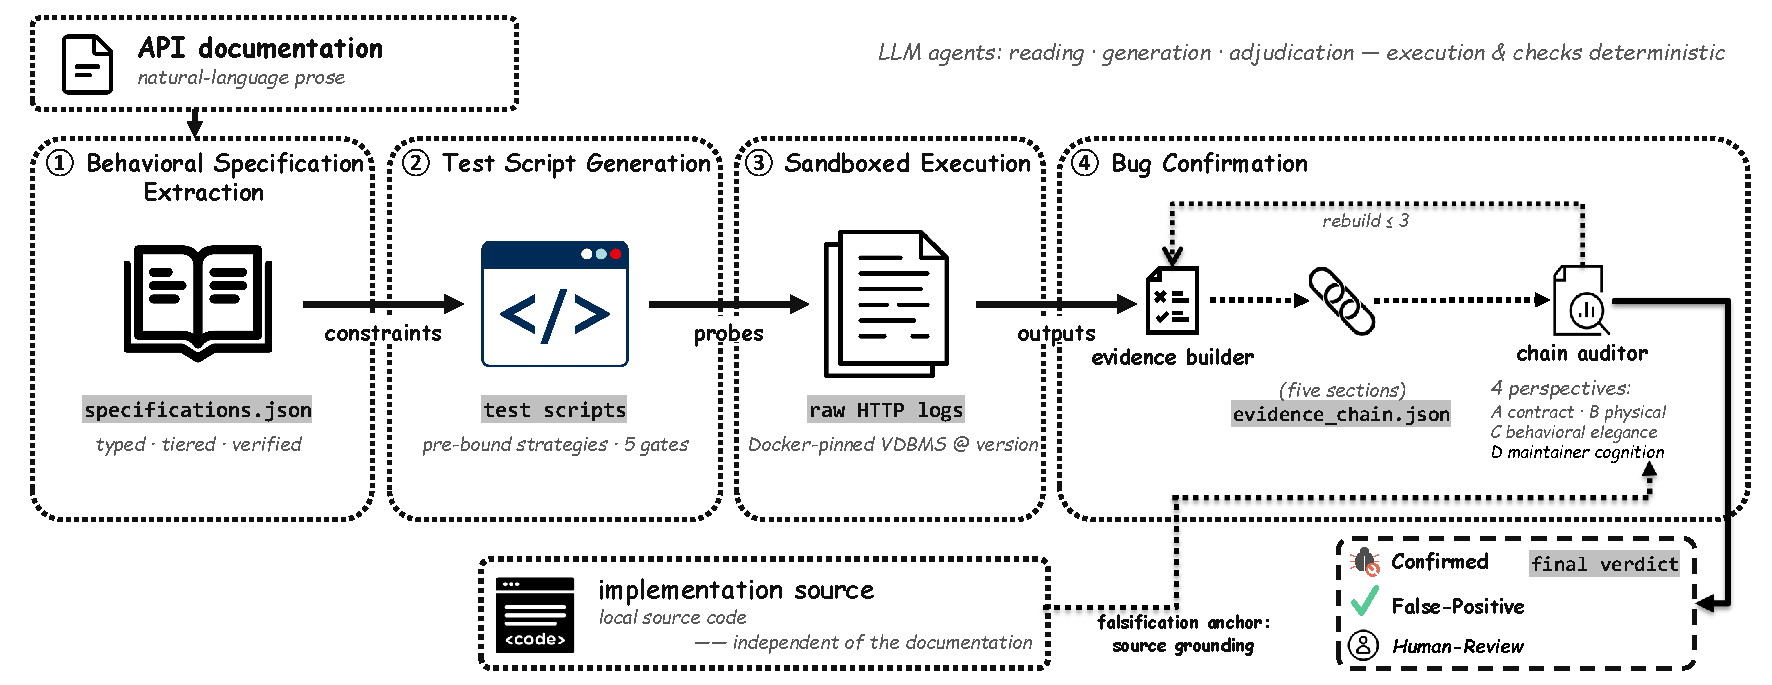
\includegraphics[width=\textwidth]{figures/pipeline-v10}
\caption{\system{} four-stage pipeline: behavioral specification extraction, test script generation, sandboxed execution, and bug confirmation. Stage~(iv) splits evidence assembly from cross-examination: an evidence builder grounds each candidate in documentation, execution output, and implementation source; a chain auditor applies four mechanical checks and four perspectives (contract, physical constraints, behavioral elegance, maintainer cognition) with a bounded rebuild loop. The implementation source is the falsification anchor (Section~\ref{subsec:confirmation}).}
\label{fig:pipeline}
\end{figure*}

\subsection{Behavioral Specification Extraction}
\label{subsec:extraction}

The first stage converts natural-language documentation into structured behavioral specifications in two steps, each owned by a dedicated agent.

\paragraph{Knowledge extraction.}
A \emph{knowledge extractor} crawls the vendor documentation for the target and version (Crawl4AI over the documentation URL space) and writes \texttt{knowledge.json}: per-endpoint entries recording method, path, source URL, parameters, constraints, and expected responses, plus a source table tracking each page's doc version. Two self-checks gate the output---an \emph{endpoint-coverage check} against the vendor's published API surface, and a \emph{version-alignment check} requiring the documentation version to match the target's major.minor, because specifications from the wrong doc version would test the wrong system. Version alignment is a precondition rather than a post-hoc filter: when a crawled artifact disagrees with the pinned version, the versioned documentation stays authoritative.

\paragraph{Specification extraction.}
A \emph{specification extractor} reads \texttt{knowledge.json} and emits \texttt{specifications.json}: one JSON record per constraint with a unique \texttt{constraint\_id}, the endpoint, a natural-language description, a checkable \texttt{assertion} (e.g., \texttt{nprobe >= 1 \&\& nprobe <= nlist}), a \texttt{type}, an \texttt{evidence\_tier}, a \texttt{source\_url} with a \texttt{source\_verified} flag, and a \texttt{level} (endpoint or system, defined below). Three mechanisms discipline the LLM in this step:
\begin{enumerate}
  \item \emph{Constraint categorization}: every constraint is typed as \texttt{type}, \texttt{range}, \texttt{state}, \texttt{behavioral}, or \texttt{other}, which downstream determines which attack agent owns it.
  \item \emph{Evidence leveling and filtering}: each constraint carries an evidence tier---\texttt{explicit} (the documentation states it verbatim), \texttt{inferred\_from\_example}, \texttt{inferred\_from\_behavior}, or \texttt{convention}---so that test strength and report claims can be graded by how directly the documentation supports them.
  \item \emph{Source verification}: for every constraint the extractor fetches the cited \texttt{source\_url} and verifies that the page genuinely contains the asserted semantics; unverified constraints are marked and excluded from downstream reporting as bug evidence.
\end{enumerate}
In the reported Qdrant run (Section~\ref{subsec:rq1}), the stage crawled 77 documented endpoints (the coverage self-check flagged two gaps) and emitted 89 typed constraints---75 endpoint-level checkable assertions and 14 cross-request contracts (7 behavioral, 7 state-invariant); all 89 passed the schema-and-tier validation gate.

\paragraph{Endpoint-level vs.\ system-level constraints.}
Each constraint carries a \texttt{level}: \emph{endpoint} or \emph{system}. The criterion is observational, not syntactic---it classifies the evidence that proves a violation, not the effort of constructing the state in which the violation occurs: \emph{what kind of observation is needed to prove that this constraint has been violated?} A constraint whose violation is decidable from a single request/response pair (an out-of-range parameter accepted, a malformed type tolerated, a coupling silently violated inside one response) is endpoint-level, even when elaborate setup is required to reach the violating request; a constraint whose violation is only decidable by relating observations across requests or against evolved system state (a stale coupling that must be detected by comparing behavior before and after a transition) is system-level. The level determines the generation path in stage~(ii).

\paragraph{Example (\#10369, stage i).}
The extractor distills the \texttt{/points/recommend} documentation---``the other collection [in \texttt{lookup\_from}] should have the same vector size as the current collection''---into constraint \texttt{qdrant\_state\_recommend\_001}: assertion ``\texttt{lookup\_from} collection must have same vector size as target collection,'' type \texttt{state}, tier \texttt{explicit}, source verified against the v1.19.0 API reference. The violation is observable in a single response (level \texttt{endpoint}), but the constraint surface---a coupling between two collections' live schemas---matches no pre-bound strategy, which routes its test to scenario construction in stage~(ii).

\subsection{Test Script Generation}
\label{subsec:generation}

Three attack agents---\emph{boundary}, \emph{state}, and \emph{semantic}---turn specifications into executable Python probes. Each agent owns a registry of \emph{built-in test strategies}, pre-registered with trigger conditions and oracle templates: boundary strategies probe values at and beyond the documented bounds (\emph{boundary value}), wrong JSON types (\emph{type violation}), and the same resource addressed through two key forms (\emph{dual-key family}); state strategies build multi-request scenarios (\emph{atomicity}: partial application of an operation the documentation prescribes as all-or-nothing; \emph{teardown-race}: deletion concurrent with use; \emph{stale-coupling}: a cross-object reference left dangling by a transition); semantic strategies check the documented meaning of a response rather than its shape (\emph{error-diagnostic quality}: the status code is right but the message misleads; \emph{contract behavior}: accept/reject semantics of a documented parameter).

\paragraph{Pre-bound strategies.}
Strategy selection is not left to the LLM at generation time. For every constraint, strategies are \emph{pre-bound} deterministically: a registry of strategy-trigger mappings---each entry a tuple of (strategy, trigger predicate over the constraint's fields)---is matched against the constraint's type, level, and assertion surface. A constraint may trigger several strategies and the agent generates for each; a constraint that triggers none falls through to scenario construction (below). Because the mapping is a pure function of the constraint record, the (constraint, strategy) pairs are reproducible from \texttt{specifications.json} alone. For each applicable strategy the attack agent then generates concrete test scripts with an inline \emph{oracle line}---a machine-checkable assertion about the expected response---which removes a degree of freedom in which the LLM could drift.

\paragraph{Level-split generation.}
The constraint level routes generation along three paths. \emph{Endpoint-level} constraints with an applicable pre-bound strategy are tested directly: the strategy instantiates request templates around the violation surface. \emph{System-level} constraints always go through \emph{scenario construction}: the agent must first build the state in which the constraint binds (collections created, points upserted, indexes built, states transitioned), then evaluate the assertion against that live state on every request, in both directions of any state transition. A constraint of either level that matches no pre-bound strategy also falls through to scenario construction, the general path for surfaces the registry does not cover.

\paragraph{Example (\#10369, stage ii).}
Constraint \texttt{qdrant\_state\_recommend\_001} matches no pre-bound strategy (cross-collection dimension coupling is not a range or type surface), so the state agent constructs the scenario: with a main collection of vector size~4 holding three ids, and a lookup collection of size~4 holding id~101, \texttt{recommend positive=[101]} with \texttt{lookup\_from} must return 200; after the lookup collection is deleted and recreated under the same name at size~8 (points upserted at size~8 with \texttt{wait=true}), the same \texttt{recommend} \emph{must} be rejected with 400 and a dimension-mismatch error. The oracle line encodes both directions.

\paragraph{Five generation gates.}
Every generated script passes five gates before it may execute: \texttt{py\_compile}; an existing \texttt{constraint\_id} in the structured contract; a risky-pattern scan (missing safe-request wrapper, swallowed exceptions); a cross-DB contamination check against a signature fingerprint table (no helper code copied from another vendor's environment); and a pre-execution check that the oracle line matches the response shape the endpoint returns. A failing script is regenerated; only passing scripts reach the sandbox.

\subsection{Sandboxed Execution}
\label{subsec:execution}

A dedicated executor runs every passing script from the host Python runtime against a Docker-pinned instance of the target at the tested version---no code executes inside the container other than the database itself. Each script writes its raw HTTP request/response pair to a log plus a completion marker created only after the log is flushed, and per-batch marker counts are reconciled, so an interrupted batch is detectable and re-runnable. The sandbox lets a candidate bug reproduce under a clean probe, and the raw records become the behavioral evidence consumed downstream.

\paragraph{Example (\#10369, stage iii).}
The scenario script executes: the initial \texttt{recommend positive=[101]} against the size-4 lookup collection returns 200; after delete-and-recreate at size~8, the same request is issued. The log pair (request, response) for both steps is written and marked.

\subsection{Bug Confirmation}
\label{subsec:confirmation}

The final stage decides, for each candidate violation, whether it is a bug. Rather than a single LLM judgment, confirmation is split into an \emph{evidence builder} that assembles the evidence and a \emph{chain auditor} that cross-examines it---a builder/judge separation with an explicit rebuild loop.

\paragraph{Evidence builder, phase 1: execution evidence and document verification.}
The builder reads the specification, the script, and the execution output, and checks four things: (1)~whether the test outputs align with the specification's assertion; (2)~whether the cited documentation actually contains the claimed semantics (content consistency, independent of the extractor's earlier verification); (3)~reproducibility and HTTP semantics---whether a $2xx$ carries a business error code or a $4xx/5xx$ is clean, and whether the observation is stable across scripts; (4)~the trace of the evidence chain, \emph{contract $\rightarrow$ doc $\rightarrow$ script $\rightarrow$ log}, flagging any broken link.

\paragraph{Evidence builder, phase 2: source grounding.}
The builder then greps the local clone of the implementation at the pinned version for parameter and error-code keywords, traces the relevant call chain, and records a \texttt{verification\_outcome}: \texttt{validation\_absent} (no check the documentation promises), \texttt{validation\_present}, \texttt{by\_design\_in\_source}, \texttt{not\_found\_in\_source}, or \texttt{webfetch\_shallow}. The output is a five-section \texttt{evidence\_chain.json}: document verification, execution evidence, contract grounding, chain trace, and source grounding---each section labeled with its evidence source (doc, behavior, source).

\paragraph{Chain auditor: four checks, four perspectives.}
The auditor applies four mechanical checks---\emph{completeness} (all five sections non-empty), \emph{consistency} (contract, documentation, log, and source aligned), \emph{self-consistency} (no contradictions), and \emph{correspondence} (the primary observation matches the specification). A chain that fails a check is sent back for rebuild (at most three retries). Surviving chains are then cross-examined from four perspectives:
\begin{itemize}
  \item \textbf{A~Contract}: does the chain's quoted contract text ground the assertion (run as a mechanical containment check)?
  \item \textbf{B~Physical}: do the objective constraint classes of the observed behavior hold? Seven classes---numeric lower bounds on count/size/limit-class parameters, closed enum sets, mutually exclusive parameters, type tautologies, same-family inconsistency, interface asymmetry across REST/gRPC/SDK faces, and (strongly qualified) HTTP response semantics---constitute violations \emph{without contract endorsement}: a limit parameter accepting zero is an objective violation even if no contract row states a bound. An ef/nprobe-class carve-out applies where the source documents a negative-sentinel convention.
  \item \textbf{C~Behavioral elegance}: may the implementation refuse the bug reading? Only an \emph{explicit} by-design may refute---the source excerpt must contain intent evidence (a code comment or docstring, e.g., ``\texttt{// intentionally}'', ``\texttt{we don't guarantee}'') or a maintainer-cognition quote must declare the same-class phenomenon intended. Bare structural inference (``no validation is present,'' an uncommented default branch) is recorded as a \emph{weak refutation} and routed to human review rather than silently closing the case.
  \item \textbf{D~Maintainer cognition}: does \texttt{developer\_cognition.json}, distilled from the target's historical issues and PRs (what the project treats as a bug and what it treats as intended), support either reading? Hits must match at phenomenon level (parameter-class or behavior-class isomorphism), never by word overlap, and cognition is a statement of maintainer attitude, not evidence---it may decide a contract-neutral gray zone but may not fill in missing execution observations.
\end{itemize}
The verdict is three-valued: \textsc{Confirmed}, \textsc{False-Positive}, or \textsc{Human-Review} (evidence insufficient, source unlocatable, or a contract/source conflict a human must reconcile---routed to the review queue rather than silently resolved, and such cases lie outside the forced-verdict rates of Section~\ref{sec:eval}). Aggregation is fixed: a contract violation confirms and cannot be overturned by source-side doubt; an explicit by-design refutes; objective-constraint violations confirm contract-neutral cases; everything else goes to human review. The rule is deliberately asymmetric, and that asymmetry is a design position rather than a claim of precision: only explicit intent evidence may refute, and anything unsettled routes to a human instead of closing. An LLM-derived oracle is expected to over-report, and the protocol keeps that over-reporting visible to a reviewer rather than suppressing it at the cost of discarding real defects. Section~\ref{sec:limitations} states the basis for the trade and what it costs. The D perspective is fed by a separate \emph{bug-shape extractor} that mines the target repository's historical issues and merged PRs into developer-cognition patterns; the implementation source is the falsification anchor of Section~\ref{subsec:overview}---it is independent of the documentation the specification was read from, and it is consulted both to ground by-design claims in verbatim intent evidence (C) and to locate the validation whose absence the contract predicts.

\paragraph{Example (\#10369, stage iv).}
The chain records: document verification PASS (the size-coupling sentence is in the v1.19.0 reference); execution evidence---200 while consistent, 200 with silently wrong scores after recreate at size~8, reproducible; contract grounding quoting \texttt{qdrant\_state\_recommend\_001}; chain trace unbroken; source grounding locating the dimension check on the direct path but absent on the \texttt{lookup\_from} path. The auditor's four checks pass; the four perspectives concur; verdict \textsc{Confirmed}. The upstream maintainer accepted the issue.

\paragraph{Implementation.}
\system{} runs as a multi-agent pipeline on an agentic coding runtime, each agent defined by a task-structured role prompt, all dispatched to a single LLM backbone (GLM) under vendor default sampling. Source grounding uses a clone of each target at the pinned version; the clone is the only authority for what the implementation does. Wall-clock per target is dominated by source grounding and live re-probes rather than raw LLM latency.

\section{Evaluation}
\label{sec:eval}

\subsection{Experimental Setup}
\label{subsec:setup}

We evaluate \system{} on three production VDBMSs---Milvus, Qdrant, and Weaviate---with each target's documentation, Docker image, and source clone pinned per tested version. The candidates span Milvus v2.3.0, v2.6.10, v2.6.12, v2.6.16, v2.6.17, v2.6.19, and v3.0.0; Qdrant v1.12.1, v1.18.0, v1.18.1, v1.18.2, v1.18.3, and v1.19.0; and Weaviate v1.37.4, v1.38.0, and v1.38.2. Every candidate is probed against the version its report names; the RQ3 reach probes additionally use Qdrant v1.18.0 (the instance the reported run's registrations came from) and v1.4.0 (the reverse direction). All agents run on one LLM family (GLM) under vendor default sampling, disclosed as a limitation (Section~\ref{sec:limitations}). Cost profile, measured from the full Qdrant run whose process ledger Section~\ref{subsec:rq1} reports: $\approx$67 active hours across five calendar days, $\approx$860 sandboxed script executions (median 1--2\,s each---the LLM agents dominate), and $\approx$70M input / 4.9M output tokens for the orchestrating session alone, a lower bound since parallel attack-agent sessions are excluded. Ground truth is maintainer adjudication (protocol in Section~\ref{subsec:rq1}). We ask three questions:
\begin{description}
  \item[RQ1 (detection effectiveness):] what documentation-implementation bugs does \system{} detect in real-world VDBMSs, as maintainer-adjudicated numbers?
  \item[RQ2 (false-positive interception):] how effective is the bug-confirmation stage (evidence builder + chain auditor) at intercepting false positives, and where do the survivors and misjudgments come from?
  \item[RQ3 (comparison with the existing approach):] how many bugs detected by \system{} can the crash-oracle approach (VDBFuzz) reach, and vice versa?
\end{description}

\subsection{RQ1: Bug Detection Effectiveness}
\label{subsec:rq1}

\paragraph{Collection protocol.}
Candidates confirmed by the pipeline are submitted as issues to the target projects' trackers. A submission counts as \emph{confirmed} when maintainers label it a bug, acknowledge it, or merge a fixing pull request, or when it is tracked to an existing issue maintainers treat as a genuine defect; as \emph{false positive} when labeled by-design or closed as not reproducible; and is additionally recorded as \emph{duplicate-tracked} when someone else had already reported it---orthogonal to the confirmed/false-positive axis rather than a third outcome. Every submission's current state---labels, closing comments, and merged-PR cross-references---was re-verified as of September 2026; the per-case ledger (system, version, issue number, adjudication status, duplicate flag, for all 81 adjudicated plus the 49 unadjudicated submissions) is included in the replication package (\texttt{rq1/ledger}). Adjudication is treated as revisable rather than final: one candidate initially counted as a fixed true positive was disproved by our own seven-version re-probe and reclassified (Section~\ref{sec:limitations}).

Table~\ref{tab:yield} reports the resulting ledger. Of 81 adjudicated candidate issues submitted upstream across the three systems, maintainers confirmed \textbf{51} as real bugs (63.0\% of adjudicated submissions); 30 submissions were adjudicated as false positives. A further 49 submissions are unadjudicated (Milvus 18, Qdrant 11, Weaviate 20)---still awaiting a maintainer verdict, or withdrawn by us without one---and are excluded from every rate we report. The seeded anchor of Section~\ref{subsec:rq2} bounds the direction of the screening this exclusion embodies: never-submitted registrations confirm at 0.594, a point estimate below the adjudicated pool's 63.0\% (the intervals overlap; the anchor bounds direction, not a significant difference). The two rates come from different arbiters, and for the anchor from a different protocol on pre-audit packs, so the bare point estimates are not like-for-like and we report the protocol-matched pairs instead. Under the stricter A/B/D rule the anchor reads 19/32 (0.594), and the submitted pool's strict readings are its forced (27/51) and joint (33/51) confirmations on the bug pool, which bracket it and so leave that pairing's direction undetermined; under the deployed protocol the anchor reads 31/32 (0.969) against the submitted pool's 48/81 (0.593), that being the full stage's confirmed-candidate share under the same convention, and there the never-submitted stream is the higher of the two. The pairing that does resolve the direction therefore places the submitted pool below the never-submitted stream, so the 0.594-versus-63.0\% contrast should be read as a directional bound rather than as evidence that screening selected stronger candidates; the unadjudicated submissions themselves---a mix of open verdicts and our own withdrawals---admit no bias estimate.

\begin{table}[t]
\caption{Submission ledger (maintainer-adjudicated, as of September 2026; accumulated across the earlier GLM-5.2 mining rounds---sixteen per-version campaigns, February--August 2026; the reported GLM-5.3-Flash run postdates the pool and contributed none of the 81; submissions still awaiting adjudication are excluded). Confirmed = maintainer-confirmed real bugs; Fixed = fixed via merged PR; duplicate-tracked = an earlier third-party report already covers the issue.}
\label{tab:yield}
\small
\begin{tabular}{@{}lrrrr@{}}
\toprule
Target & Adjudicated & Confirmed & Fixed & FP \\
\midrule
Milvus & 43 & 29 & 11 & 14 \\
Qdrant & 28 & 14 & 9 & 14 \\
Weaviate & 10 & 8 & 3 & 2 \\
\midrule
Total & 81 & 51 & 23 & 30 \\
\bottomrule
\end{tabular}
\end{table}

\textbf{Bug status.} Of the 51 confirmed bugs, 23 have been fixed via merged PRs on our submissions; 18 remain open with maintainer acknowledgment; 7 were closed without a fix after acknowledgment. The remaining 3 (Milvus \#52308, \#52310, \#52312) are defects someone else had already reported; all three were closed as completed once that earlier report was fixed upstream, and they are flagged duplicate-tracked in the ledger rather than counted in our fix column. The fix count validates that the confirmed bugs are actionable defects rather than report inflation. On the other side of the ledger, 27 of the 30 adjudicated false positives were closed as intended behavior and 3 as not reproducible.

\textbf{Upstream acceptance.} The three projects share no severity-label scheme, so we report the acceptance signals they do attach: 50 of 51 confirmed bugs carry an official \texttt{bug} label (the exception, Qdrant \#9524, is validated by its merged fix PR), 25 of 29 Milvus bugs carry \texttt{triage/accepted}, and 5 of 14 Qdrant bugs \texttt{accepted}.

\textbf{Fix nature.} To validate that ``fixed'' reflects genuine code repairs rather than documentation tweaks or test additions, we classify every merged fix PR by its changed files. All 23 fixed bugs have a locatable merged fix PR; every one of the 23 modifies implementation code, 15 also add regression tests, and none is documentation-only. As a check on the classifier itself, applying it to the fix PR of the disproved \#9149 (Section~\ref{sec:limitations}) correctly identifies that PR as test-only---exactly matching the seven-version re-probe that reclassified the candidate, which now sits among the 30 adjudicated false positives rather than the 51.

\textbf{Bug categories.} We group the confirmed bugs into eight named bug patterns, each defined by what the documentation prescribes and how the implementation deviates (Table~\ref{tab:bug-patterns}). The taxonomy is dominated by the acceptance family: \textsc{Silent-Accept}, \textsc{Type-Coercion}, and \textsc{Silent-Ignore} together account for 37 of 51 bugs (72.5\%)---all shapes in which the system returns success while violating a documented constraint. Two patterns concentrate per system: \textsc{Type-Coercion} occurs only in Milvus (its REST layer silently converts types and substitutes invalid enum values where gRPC rejects), and the \textsc{Result-Incorrectness} cluster in Qdrant centers on approximate \texttt{count} under-counting. One boundary: the \textsc{Result-Incorrectness} bugs sit outside the assertion framework by construction---no documented accuracy contract bounds approximate behavior---so they entered the ledger on maintainer adjudication alone rather than through a contract assertion. All five are in the RQ2 pool, where the documentation's own reliability disclaimer (Section~\ref{subsec:rq2}) makes them, at four of the twelve misses, tied with the unconsumed-top-level-field family for the largest block of the full stage's residual misses; because that family is unreachable by the framework, we also report the in-class reading---the stage confirms 38 of the 46 candidates whose class the framework targets (0.826, against 0.765 over all 51)---so the headline is not carried by a class the method does not address.

\begin{table}[t]
\caption{Bug patterns over the 51 confirmed bugs. Representative = one confirmed issue per pattern; the pattern rows include the three duplicate-tracked bugs.}
\label{tab:bug-patterns}
\small
\begin{tabular}{@{}p{0.34\columnwidth}rp{0.42\columnwidth}@{}}
\toprule
Pattern & \# & Representative \\
\midrule
\textsc{Silent-Accept} & 25 & \texttt{nprobe=0} accepted (Milvus \#49823) \\
\textsc{Type-Coercion} & 8 & string$\to$Int64 primary key (Milvus \#52308) \\
\textsc{Result-Incorrectness} & 5 & \texttt{count} under-counts (Qdrant \#10120) \\
\textsc{Silent-Ignore} & 4 & \texttt{strictGroupSize} ignored (Milvus \#52325) \\
\textsc{Weak-Diagnostic} & 3 & HTTP 500 for standalone ops (Qdrant \#9421) \\
\textsc{Stale-Coupling} & 2 & \texttt{lookup\_from} dimension bypass (Qdrant \#10369) \\
\textsc{Doc-Spec-Gap} & 1 & OpenAPI missing size bound (Qdrant \#9942) \\
\textsc{Other} & 3 & zero-length vector accepted, then panic on later search (Qdrant \#9045; one of three) \\
\bottomrule
\end{tabular}
\end{table}

\textbf{Process ledger of one complete run.} The upstream ledger reports outcomes; one complete end-to-end run of \system{} on Qdrant v1.18.0 exhibits the funnel behind them (recorded under that run's pre-review protocol, whose verdict vocabulary predates the \textsc{Human-Review} channel of Section~\ref{subsec:confirmation}): all 66 feature blocks mined to closure; 119 chain verdicts (per-evidence-path), 70 defect-confirming and none unresolved, resolving to 96 distinct candidates of which 60 confirm defects; the novelty gate partitioning those 60 into 19 novel, 11 already covered by merged upstream fix PRs, 5 by-design, and 25 pending; and the 44 that are neither covered nor by-design (19 novel + 25 pending) passing deduplication and family merging to register five new defect numbers. Those last two steps are many-to-one without a maintained per-step count, so the funnel is reported at its two measured points, not as a complete chain of subtractions; the artifact's defect registry records each registration and its merged candidates.

\textbf{External corroboration.} Two confirmed defects were fixed upstream within the following releases---independent confirmation; a third (a malformed-archive request answered with a server error disclosing internal filesystem paths) rests on our own reproduction, still live on the latest release four-for-four at time of writing---reproducibility, not independent adjudication. The gate's own caveat: two of its by-design matches were word-level false positives that manual review overrode; lexical novelty matching is the funnel's weakest link. The submission ledger of Table~\ref{tab:yield} is the sum of sixteen per-version campaigns accumulated since early 2026 and predates this run, contributing to it additively rather than being contained in it.

The 30 adjudicated false positives are not waste: they are exactly the population on which RQ2 measures---and remeasures---the confirmation stage's interception capability. Our measurement design---maintainer adjudication as ground truth, explicit duplicate handling, a disclosed submission-filtered pool, and pool-internal recall---sits in the bug-finding-evaluation tradition~\cite{klees18,magma21}. One caveat follows from how that population arose: submission decisions were made per candidate by the authors after novelty screening and manual review (no deterministic submission rule), so the 81-candidate pool is a submission-filtered subset of the pipeline's confirmed output rather than a random sample of it. The induced bias is conservative for suppression---weak candidates were screened out, so raw-stream suppression is likely \emph{higher} than measured---while the 63.0\% precision inherits the human decision's selectivity; the recall direction is anchored below in Section~\ref{subsec:rq2}.

\subsection{RQ2: Effectiveness of False-Positive Interception}
\label{subsec:rq2}

The two headline results are earned under different configurations. The RQ1 ledger is the operational pipeline's cumulative output: it ran unblinded with the judgment-side threats of Section~\ref{sec:limitations} live, and author-side novelty screening and the submission decision sat in the loop. Everything in this subsection instead re-adjudicates the pool that ledger produced, under blinding and with no human in the automated arms. The two measure different layers, and neither is the complement of the other. All 81 adjudicated submissions originate from the earlier mining rounds (Section~\ref{sec:limitations} records the serving split): the reported GLM-5.3-Flash run postdates the pool and contributes to the ledger additively. The pool itemizes cleanly at target granularity: its 81 submissions distribute over sixteen mining targets (seven Milvus, six Qdrant, and three Weaviate versions, the list Section~\ref{subsec:setup} gives), each a bounded mining session whose submissions fall within a single month between February and August 2026, with one target (Qdrant v1.18.1) spanning two. What we cannot reconstruct retroactively is the per-session strategy and rule configuration inside each target, so the ledger is the sum of sixteen per-version campaigns rather than one configuration's output. The RQ2 measurement does not depend on that provenance, since every candidate is re-adjudicated from scratch under the frozen protocol on rebuilt packs---it bears on the RQ1 ledger, which is disclosed as the human--machine pipeline's cumulative output. To anchor the direction of the submission filter, we re-adjudicated 32 candidates seeded from the reported Qdrant run's registrations that never entered the 81-pool (four further registrations, tracked to a ledger issue, were excluded from the sample), three independent runs each, under a \emph{stricter} protocol than the full stage's: perspectives A, B, and D only, where D here is the builder's source-grounding face rather than the maintainer cognition the full stage reads---with binary verdicts and unresolved cases closed as false positives rather than routed to review. The blinded arm re-confirms 19/32 (0.594, Wilson [0.423, 0.745]; unanimous on 26). Because that rule set force-closes what the full stage would route, 0.594 is a floor; re-running the same 32 packs under the deployed protocol---four perspectives, three-valued verdicts, routed cases counted as confirmed---gives 31/32 (per-run 31, 32, 31; 22 cases unanimous), so the pair brackets the sample the way the three readings bracket the main pool. We keep 0.594 in the text because it does not depend on the counting convention: it is the reading a reviewer who distrusts the routing rule would still have to accept. Neither figure is a recall measure---these candidates never reached maintainers and have no adjudicated ground truth---and the deployed-protocol figure is high partly because routing counts as confirmation and partly because these pre-audit packs carry weaker contract rows, which pushes cases off the contract perspective and onto the objective-constraint one. The anchor was also measured on the original packs before the audit, so its absolute value is not comparable to the rebuilt-package numbers below. What it establishes is that the pipeline's non-submitted registrations contain adjudicable, frequently-confirmable candidates rather than chaff---the submission filter selects among live candidates rather than inflating pool confirmability by construction. Throughout, we keep two senses of ``false positive'' apart: a \emph{false-positive candidate} is one of the 30 maintainer-adjudicated non-bugs, whereas \textsc{False-Positive} (small caps throughout) is the verdict the stage returns; suppression rates are computed over candidates, and a \emph{leak} is a candidate the stage confirms; a \emph{pack} is one candidate's frozen evidence bundle, a \emph{case} is one candidate in the pool, and a \emph{case judgment} is one candidate as judged in one run---243 pooled across the three runs. A \emph{case-agreement rate} is the share of the 81 cases on which all three runs returned the identical verdict label, and a case is \emph{routed} when at least one of its three runs returns \textsc{Human-Review}; the routed queue we hand-adjudicate below is the subset the majority also confirms.

\textbf{Measurement design: audit, rebuild, protocol alignment.}
The measurement went through two corrections, and we report all three layers because each isolates one variable. \emph{Layer 0, the shipped packs}: an audit of the originally assembled 81 packs against the documentation pages they cite---a mechanical assembly pass (endpoint filtering, provenance stripping) followed by per-pair verification whose verdicts, evidence tiers, and notes ship as records---found that 43.3\% of their 134 distinct (constraint, cited-page) pairs had no support on the page, a further two pairs were over-strong relative to their page, and 32\% of all constraint rows addressed an endpoint unrelated to the candidate's own; the four packs carrying assembler provenance notes leaked adjudication-adjacent annotations into judge materials. Every defect traced to the assembler (a per-vendor fixed-version contract substitution, parameter-name rather than endpoint matching, and undocumented implementation-private constants read as contract), not to the confirmation stage. \emph{Layer 1, rebuilt packs}: we rebuilt all 81 packs from version-pinned documentation and the tested version's own OpenAPI artifact---each surviving constraint row carries its page citation, a source-type label (\emph{documentation} vs.\ \emph{structured spec}), an evidence tier, and a gate record; the four leaked provenance notes were removed before any re-adjudication. The rebuilt packs contain 674 constraint rows out of 2{,}106 originally assembled (the surviving count numerically coincides with the endpoint-filtered count that follows): endpoint filtering removed 674 rows and evidence verification removed 463; of the 969 survivors, 667 were kept as rebuilt contract rows and the 302 rows of 12 packs whose contract sections were replaced wholesale by case-level archaeology were dropped, with seven of those archaeology packs each retaining a single assertion row (667~+~7~=~674), typed as 22 \texttt{explicit} and 652 \emph{inferred-from-behavior}. The audit verified citations, not observation payloads, and that boundary is worth recording: four candidates reproduce the filed report's parameter shape rather than the shape the API consumes---three with their grouping knobs inside a nested \texttt{groupParams} object, which is not a field of the REST v2 search request (its binder reads flat \texttt{groupingField}, \texttt{groupSize}, and \texttt{strictGroupSize}), and one with a top-level \texttt{shardsNum} where only \texttt{params.shardsNum} is read---so in each the unknown key is dropped whole and the recorded observation shows that drop rather than the validation gap the report describes. The three group-by candidates are nevertheless true positives: the maintainers reproduced all three with the corrected payload and fixed them together in a merged PR, so their confirmations rest on that reproduction and fix rather than on our own observations. The \texttt{shardsNum} case is the leak Section~\ref{sec:limitations} already counts, and its observation is correspondingly weak. 21 packs carry no surviving contract row that covers their endpoint---14 of the 51 true bugs sit in these packs, the basis of the evidence-absent and weak-evidence strata (the weak-evidence packs retain a single row, but one the audit flagged as behavioral inference rather than a normative statement about the constrained field) below---including two of the four leak cases whose only pack-level ``support'' had been the leaked annotation. \emph{Layer 2, protocol alignment}: the judging protocol was aligned with the deployed chain-auditor rules after we found our first re-adjudication protocol still carried two pre-deployment rules that the audit had not touched but that suppressed recall by construction---by-design refutation accepted bare structural inference (``no validation is present'') rather than requiring verbatim intent evidence, and ``validation present'' counting as non-defect evidence even when no contract row covered the observed face. The deployed protocol requires intent evidence to be quoted verbatim, treats the seven objective constraint classes of Section~\ref{subsec:confirmation} as violations that need no contract endorsement, and routes unresolvable cases to an explicit \textsc{Human-Review} verdict instead of forcing \textsc{False-Positive}. On the observation side, a mechanical scan of all 81 rebuilt packs found 19 expectation-flavored phrases in observed sections, all inside verbatim server responses (``it should be in range [1, 16384]''); zero expectation framing was added by assembly, so no sanitization was applied and none was needed.

\textbf{Arms and adjudication.}
Nine judge configurations follow, distinguished only by what the judge sees and which rules it applies (Tables~\ref{tab:rq2-matrix},~\ref{tab:rq2-single}): contract core (pack only, contract assertions as the sole standard---a binary verdict on pack material alone: confirmed only where an observation explicitly violates a pack contract assertion, no source access and no human-review channel, with unresolved cases resolved to false positive), full stage (the same pack and pinned source clone plus the maintainer-cognition materials, judged under the four-perspective protocol and its aggregation), source-only (the confirmation stage's source-forensics step operating alone---the same pack and source materials with no cognition access, judged with the same three-valued verdict space and scored under the same convention as every other arm; the ``source-only'' rows in the tables), flat judge (a single prompt over the same packs and sources but without the assembled evidence chain the auditor reads, cognition access likewise excluded), the two component controls (the flat judge with only its output-schema line corrected, and the flat judge additionally bound to the full stage's fixed aggregation rule, both without perspective vocabulary or evidence-chain sections), the full stage with the implementation source withheld (``full, no source''; every rule sentence intact, the clone removed and the source channel closed), the full stage with its aggregation removed (``full, no aggregation''; the four perspectives kept, the judge weighing them itself), and source-only on a second backbone (``source-only-Qwen''). Every configuration re-adjudicates the full pool of 81 candidates (51 real bugs + 30 false positives) in three independent runs: identical packs, default sampling, no access to adjudication labels or issue history except the maintainer-cognition materials the full stage reads as perspective D (historical patterns mined in August 2026, before the re-adjudication and scoped in Section~\ref{sec:limitations}), and every case judged in every run. The verdict is three-valued (\textsc{Confirmed}/\textsc{False-Positive}/\textsc{Human-Review}, Section~\ref{subsec:confirmation}); \textsc{Human-Review} cases count toward \textsc{Confirmed} in every rate below. This is the deployment's operating point rather than a convenience: the protocol routes a case it cannot settle instead of closing it as a false positive, and the deployment reports what it routes---a routed case goes upstream unless a reviewer finds it egregiously wrong. We refer to this as the deployment's counting convention; it is the reading that matches the deployment's policy and needs no adjudicator, because the deployment reports what it routes. The forced reading below is equally mechanical---the same verdict files, re-scored---and is the conservative floor; the hand-adjudicated readings, including the independent re-adjudication we report there, are strict-review sensitivities that sit between the two. We report both components where the distinction matters; Appendix~\ref{app:prompts} quotes both the full-stage and the flat-judge prompts. Unless a row or a sentence says otherwise, every rate below is computed on the rebuilt, cleaned packs, with each configuration's three runs reduced by majority vote and \textsc{Human-Review} counted as confirmed.

\begin{table}[t]
\caption{Confirmation-stage ablation over the 81-candidate pool (51 real bugs, 30 false positives) on rebuilt packs: the contract core (pack only) and the full stage (pack plus the structured four-perspective protocol), each in three independent runs with majority vote ($\geq$2/3). \textsc{Human-Review} verdicts count as confirmed (Section~\ref{subsec:confirmation}).}
\label{tab:rq2-matrix}
\small
\begin{tabular}{@{}lrrrr@{}}
\toprule
Run & TP & FP leaked & FN missed & TN intercepted \\
\midrule
core, run 1 & 9 & 1 & 42 & 29 \\
core, run 2 & 9 & 1 & 42 & 29 \\
core, run 3 & 9 & 1 & 42 & 29 \\
core, majority & 8 & 1 & 43 & 29 \\
\midrule
full, run 1 & 40 & 8 & 11 & 22 \\
full, run 2 & 38 & 9 & 13 & 21 \\
full, run 3 & 35 & 11 & 16 & 19 \\
full, majority & 39 & 9 & 12 & 21 \\
\bottomrule
\end{tabular}
\end{table}

\begin{table}[t]
\caption{Independent arms over the same 81 rebuilt packs: the source-only judge sees each pack and the pinned source clone; the flat judge is a single prompt with the same inputs and no perspectives, chain sections, or aggregation rule; the two \emph{flat judge $+$} arms decompose the flagship gap (Section~\ref{subsec:rq2})---``schema fix'' corrects only the flat dispatch's output-schema line, which declared a binary verdict field while its v3 supplement mandates three-valued verdicts, and ``aggregation'' additionally binds the judge to the full stage's fixed aggregation rule with no perspectives or chain sections; ``full, no source'' is the full stage with the implementation source clone withheld and the source channel closed (Section~\ref{subsec:rq2}), every rule sentence left intact; ``full, no aggregation'' is the full stage with its aggregation text removed---the dispatch carries two such blocks, an earlier conservative rule and the deployed fixed one, and both were excised---so the judge reads the same four perspectives over the same materials and weighs them itself; source-only-Qwen re-runs the source-only arm on a second backbone, whose three runs are collapsed to its majority row. Majority vote ($\geq$2/3); core and full majorities repeated for reference.}
\label{tab:rq2-single}
\small
\begin{tabular}{@{}lrrrr@{}}
\toprule
Run & TP & FP leaked & FN missed & TN intercepted \\
\midrule
source-only, run 1 & 35 & 7 & 16 & 23 \\
source-only, run 2 & 38 & 11 & 13 & 19 \\
source-only, run 3 & 37 & 5 & 14 & 25 \\
source-only, majority & 36 & 8 & 15 & 22 \\
flat judge, run 1 & 30 & 6 & 21 & 24 \\
flat judge, run 2 & 31 & 3 & 20 & 27 \\
flat judge, run 3 & 27 & 6 & 24 & 24 \\
flat judge, majority & 30 & 4 & 21 & 26 \\
flat judge $+$ schema fix, run 1 & 29 & 6 & 22 & 24 \\
flat judge $+$ schema fix, run 2 & 37 & 6 & 14 & 24 \\
flat judge $+$ schema fix, run 3 & 34 & 0 & 17 & 30 \\
flat judge $+$ schema fix, majority & 35 & 4 & 16 & 26 \\
flat judge $+$ aggregation, run 1 & 40 & 15 & 11 & 15 \\
flat judge $+$ aggregation, run 2 & 43 & 8 & 8 & 22 \\
flat judge $+$ aggregation, run 3 & 39 & 11 & 12 & 19 \\
flat judge $+$ aggregation, majority & 39 & 12 & 12 & 18 \\
source-only-Qwen, run 1 & 32 & 10 & 19 & 20 \\
source-only-Qwen, run 2 & 36 & 7 & 15 & 23 \\
source-only-Qwen, run 3 & 39 & 8 & 12 & 22 \\
source-only-Qwen, majority & 37 & 9 & 14 & 21 \\
\midrule
contract core, majority (ref.) & 8 & 1 & 43 & 29 \\
\midrule
full, no source, run 1 & 47 & 17 & 4 & 13 \\
full, no source, run 2 & 43 & 14 & 8 & 16 \\
full, no source, run 3 & 49 & 14 & 2 & 16 \\
full, no source, majority & 48 & 16 & 3 & 14 \\
\midrule
full, no aggregation, run 1 & 34 & 2 & 17 & 28 \\
full, no aggregation, run 2 & 27 & 1 & 24 & 29 \\
full, no aggregation, run 3 & 33 & 3 & 18 & 27 \\
full, no aggregation, majority & 33 & 2 & 18 & 28 \\
\midrule
full, majority (ref.) & 39 & 9 & 12 & 21 \\
\bottomrule
\end{tabular}
\end{table}

\textbf{The contract core: suppression without semantics.}
Under majority voting the core recalls 8/51 (0.157, Wilson [0.082, 0.280]) while suppressing 29/30 false positives (0.967, Wilson [0.833, 0.994]); case-level agreement across its three runs is 96.3\% (78 of 81 cases): the three disagreeing cases are true bugs that flip between runs, each confirmed in exactly one run and outvoted two-to-one on the other two, so each per-run row counts its eight unanimous confirmations plus one run-specific flip, while the majority retains only the unanimous eight. Its single leak is a case whose rebuilt pack carries an explicit closed-set assertion the observation violates. This is the assertion-framework floor: a judge that sees only documented prose and the observation can intercept what the documentation forbids, and can do so almost perfectly stably---but 652 of the 674 surviving constraint rows are behavioral inference rather than verbatim-explicit assertions (22 are \texttt{explicit}), so the semantics violated by most true bugs enter the pack as inference, and the core has no other ground to stand on.

\textbf{The full stage: recall recovered, suppression traded.}
The structured stage recalls 39/51 (0.765, Wilson [0.632, 0.860]) at suppression 0.700 (Wilson [0.521, 0.833]) and precision 0.812. Of its 39 confirmations, 23 are \textsc{Confirmed} in all three runs; of the remaining 16, fifteen carry at least one \textsc{Human-Review} component, ten of those with a \textsc{Human-Review} majority, and four carry a minority \textsc{False-Positive}. The forced-verdict reading is $23+4=27$, the four being the minority-confirmation cases whose two \textsc{Confirmed} votes survive a minority label. The three-run case agreement is 67.9\% (55 of 81 cases), and 19.8\% of all full-stage verdicts---48 of the 243 case judgments pooled across the three runs---route to review. The suppression cost relative to the core is eight cases: six are false positives the protocol routes to a human rather than closes, and two are forced-verdict disagreements---a shardsNum acceptance whose probe value a later source reading suggests may never have bound (the binding-artifact note in Section~\ref{sec:limitations}), and a batch-delete case judged through a near-version clone. A ninth leak, an enum-closure confirmation on a parameter the implementation silently defaults, is already confirmed by the contract core---it is the core's single leak---and so adds no \emph{relative} cost. All are recorded as protocol-vs-adjudication conflicts, not measurement errors.

\textbf{Structure is a measured mechanism---and the decomposition narrows it.}
The paper's central comparison is the full stage against a flat single-prompt judge reading the same packs and sources, with no perspective vocabulary, evidence-chain sections, or aggregation rule (Table~\ref{tab:rq2-single}): the flat judge reaches majority recall 0.588 (Wilson [0.452, 0.712]) at suppression 0.867---solidly between the core and the full stage, but statistically below the full stage. Over the 81 paired cases the full stage beats the flat judge on 16 and loses on 2---each test pairs the two arms' \emph{confirmed sets} (\textsc{Confirmed} or \textsc{Human-Review} under the convention above, so a ``leak'' counts as confirmed on both sides), the discordant net therefore matches the confirmed-set difference, and here it is 48 vs.\ 34, net $+14$ (exact McNemar $p{=}0.0013$, Holm-corrected $p{=}0.0052$ across the seven paired tests in this subsection\footnote{The family is defined by construction: the seven confirmation-arm pairs on the primary pool. The seven paired tests, with raw exact $p$ and discordant nets: core-vs-flat $<0.0001$ (discordant 0/25); core-vs-source-only $<0.0001$ (2/37); core-vs-full $<0.0001$ (1/40); full-vs-flat $p{=}0.0013$ (16/2; fourth-smallest, Holm multiplier 4); source-only-Qwen-vs-flat $p{=}0.0075$ (15/3; fifth-smallest, multiplier 3, adjusted 0.023; backbone replication below); source-only-vs-flat $p{=}0.041$ (15/5); full-vs-source-only $p{=}0.39$ (8/4). Adding the subsection's three sensitivity analyses (the forced-verdict pair, the joint-vs-flat pair, and the second-family replication) to the family as a maximal ten-test set raises the flagship's adjusted value only to 0.0092; adding instead the three control pairs reported below (source-withheld-vs-full, raw $p{=}0.0004$; aggregation-vs-flat, raw $p{<}0.0001$; aggregation-vs-full, raw $p{=}0.61$) makes ten tests, places the flagship sixth-smallest and gives $0.0013\times5=0.0066$, and a maximal thirteen-test set containing both groups leaves it sixth-smallest and gives $0.0013\times8=0.0105$. The conclusion is unchanged under every extension we test.}). Decomposed by ground truth, $+9$ of that net is true positives and $+5$ is additional leakage: a true-positive-only exact McNemar on the 51 bugs gives 11/2 (raw $p{=}0.0225$), which does not survive correction within this family (Holm-adjusted 0.090, applying the flagship pair's multiplier~4; ranked as a separate family member the recall-only test would take multiplier~3 and give 0.0675, and the conclusion is unchanged under either), while the leakage-only difference is 5/0 ($p{=}0.0625$). The flagship's Holm survival therefore rests on the confirmed-set basis---the unit the deployment resolves---rather than on the recall-only comparison alone. The advantage is not an artifact of that unit: on metrics that price a confirmed false positive against a confirmed true positive, the full stage leads on both backbones. On the primary family it confirms 30 more true bugs than false positives where the flat judge confirms 26 ($F_1$ 0.788 vs.\ 0.706; Youden's $J$ 0.465 vs.\ 0.455, over the 81-candidate pool), and on the second family the same ordering holds (25 vs.\ 22; $F_1$ 0.698 vs.\ 0.651; $J$ 0.422 vs.\ 0.363)---so the direction replicates there even though the paired test above lacks the power to establish it. The margin is not uniform: on the primary family the two arms are effectively tied on $J$ (0.465 vs.\ 0.455), so the leads that carry are the net true-positive count and $F_1$, not the balanced accuracy. The flat judge in turn beats the contract core ($p{<}0.0001$), as do source-only ($p{<}0.0001$) and the full stage ($p{<}0.0001$). The ordering resolves cleanly once the component controls are slotted in---core $<$ flat $<$ flat$+$schema fix $<$ source-only $<$ flat$+$aggregation $\approx$ full, with the source withheld at 0.941 on the confirmed set but at 0.467 suppression---of which the full-vs-flat separation survives correction under every family size we test, full-vs-source-only is indistinguishable ($p{=}0.39$; the two confirmed sets differ by four cases, so that test is underpowered at this pool size), and the case-level decomposition shows the small gap is not routing-carried: of the eight cases the full stage confirms and source-only does not, six are forced \textsc{Confirmed} majorities delivered by the perspectives---three of them unanimous, on cases where the source-forensics dispatch alone finds at most one \textsc{Confirmed} run---and only two are \textsc{Human-Review}-majority confirmations; the four reverse cases are two routed true positives the full stage force-closed and two leaks, and the flat-vs-source-only step does not survive correction ($p{=}0.083$); the second-backbone source-only arm separates from the flat judge at a corrected $p$ of 0.023 (backbone replication below).

The decomposition, however, locates the mechanism precisely. Under forced-verdict-only scoring (each run's \textsc{Human-Review} verdicts re-scored as \textsc{False-Positive} and the three runs then reduced by majority again, so the reading is what the stage would decide if it had to decide), the full stage recalls 0.529 (27/51) and the flat judge 0.490 (25/51)---indistinguishable (discordant 7/3, $p{=}0.34$). The full-vs-flat separation is therefore carried by the routing channel, not by forced-verdict accuracy: the structured protocol escalates to explicit human-review decisions (15 of the full stage's 39 confirmations carry at least one \textsc{Human-Review} vote) the cases the flat judge closes by fiat, and the flat judge---which shares the three-valued verdict space but has no aggregation rule that mandates routing, and in the primary family routes only 8.6\% of its verdicts (21 of 243 pooled across its three runs)---force-closes 7 of those 15 routed confirmations as \textsc{False-Positive}. The two arms' routed queues are about equally precise---the full stage's holds 15 true bugs out of 21 and the flat judge's 8 out of 11---so on this pool they differ chiefly in how often they decline to decide, not in how well they decide when they do. On this pool, what the routing rule buys is not better forced guessing but honest escalation. Which part of the protocol supplies that rule is the question the next paragraph takes up.

\textbf{What in the protocol carries the gap.} The flat judge differs from the full stage in two things at once---the four-perspective organization and the aggregation rule---so the comparison above cannot say which one the separation belongs to. We therefore added each component to the flat judge in turn, holding the packs, the source clones, the discipline clauses, and the red lines fixed (the two ``flat judge $+$'' arms of Table~\ref{tab:rq2-single}). Both arms first correct an inconsistency in the flat dispatch, whose output-schema line declared a binary verdict field while its v3 supplement mandates three-valued verdicts; the first arm stops there, and the second additionally binds the judge to the full stage's fixed aggregation rule---expressed in the flat judge's own vocabulary, since it carries no A/B/C/D perspective labels---with no perspective vocabulary and no evidence-chain sections. The schema-only arm reaches majority recall 0.686 (35/51) at suppression 0.867: directionally above the flat judge ($+5$ net, discordant 6/1, $p{=}0.125$) but not significantly so, and with routing (7.8\%, 19 of 243 case judgments) and suppression matching the flat judge's rather than the full stage's. That arm is the baseline the flagship should be read against, since it is the flat judge with its dispatch repaired, and the full stage still separates from it---confirmed sets 48 against 39, discordant 13/4, net $+9$---but only at raw $p{=}0.049$, which enters the seven-test family eighth and takes multiplier 2 for an adjusted 0.098: the flagship's Holm-surviving separation is measured against the shipped flat dispatch, and against the repaired one it is a marginal raw result that does not survive correction. Adding the aggregation rule reaches 0.765 (39/51) at suppression 0.600---identical to the full stage on recall and indifferent on the confirmed set (discordant 9/6, $p{=}0.61$; forced-verdict recall 27/51 in both arms), significantly above the schema-only arm (discordant 2/14, $p{=}0.0042$), while routing 28.4\% of verdicts (69 of 243) against the full stage's 19.8\% (48 of 243). The recall the full stage earns over the flat judge is therefore reproduced \emph{without} the four-perspective organization, and the organization's own increment is measured in the paragraph below and is absent on this pool, though the point estimates favour it where the convention does not reach---nine leaks against the control's twelve, and a routed-queue precision of 0.714 (15/21) against 0.600 (15/25)---neither difference being significant (exact McNemar $p{=}0.45$; Fisher exact $p{=}0.54$).

\textbf{The completed two-by-two.} The controls above leave one cell of the design empty---the four perspectives \emph{without} the aggregation rule---which is why the attribution to the rule rested on a contrast the design could not complete. Filling it (``full, no aggregation'' in Table~\ref{tab:rq2-single}) settles the question. With both aggregation blocks excised and every other rule sentence intact, the four perspectives reach majority recall 0.647 (33/51) at suppression 0.933---statistically indistinguishable from the flat judge that has neither (discordant 6/5, net $+1$, $p{=}1.0$), and significantly below both the full stage (discordant 1/14, net $-13$, $p{=}0.0010$) and the aggregation-only control (discordant 3/19, net $-16$, $p{=}0.0009$). Read across the design, adding the aggregation rule moves recall in both rows (0.588 $\to$ 0.765 without perspectives, $p{<}0.0001$; 0.647 $\to$ 0.765 with them), while adding the four perspectives moves it in neither ($+3$ and not significant without the rule, $p{=}1.0$; exactly nothing with it). The perspectives' contribution over a flat judge is therefore not established on this pool---the paired difference in recall is $+0.020$, 95\% CI $[-0.108, +0.147]$, which spans zero---though the perspective-only arm sits significantly below both arms that carry the aggregation rule ($p{=}0.0010$ against the full stage, $p{=}0.0009$ against the aggregation-only control), and it is also the most precise configuration we ran (0.943, against the full stage's 0.812), which is what a reading that refuses nearly everything would look like. What the rows do share is the forced-verdict total---27/51 in the full stage, the aggregation-only control, and the perspective-only arm alike---but on inspection that is a coincidence of counts rather than a common decision core: the three arms agree on only 21 of the 27, each holding three to five cases the others do not, and their union is 33. The structure therefore changes which cases each configuration decides, and it changes that without changing how many. One disclosure bounds the reading: the control, like the rest of this subsection, ismeasured on one backbone.

\textbf{What the implementation source is for.} The control that prices the source is its removal: withholding the source clone from the full stage---every rule sentence, the four perspectives, the aggregation, and the cognition materials left intact, only the clone removed and the source channel closed---raises convention recall from 0.765 to 0.941 (48/51) and cuts suppression from 0.700 to 0.467, a net of 16 cases in the withheld arm's favour (discordant 2/18, $p{=}0.0004$). The source is not the mechanism that finds the bugs; it is the mechanism that refuses them. That much is structural rather than statistical: in the fixed aggregation the source-anchored perspective can only refute---it appears in the by-design clause and in no clause that confirms---so its votes enter a verdict only as refusals. Across the full stage's 243 case judgments it casts 41 explicit by-design refutations and 59 weak ones against 72 confirmations the aggregation never consults, and the swing when it is removed is correspondingly one-sided: keeping the channel costs nine adjudicated true bugs and refuses seven adjudicated false positives. Two limits belong with that reading. A by-design refutation must rest on verbatim intent evidence, and the 41 do not all: two record bare structural inference---an absent binding tag and an uncommented fallback chain read as intent---where the red line requires the case to route instead, and both closed their case as \textsc{False-Positive}, one of them an adjudicated true bug, which is the precise failure the rule exists to prevent. The remaining 39 carry the verbatim comment, docstring, or maintainer quote the rule demands (the per-judgment audit ships in the artifact). And the design position of Section~\ref{sec:limitations} prices a false positive as the cheaper error, whereas this is the one channel not priced that way, so the measured deployment is in this respect more conservative than its own stated position. The withheld arm is also, on the paper's own summary metrics, the stronger configuration: net true positives minus leaked false positives is 32 against the full stage's 30, and $F_1$ is 0.835 against 0.788. We do not read that as a defect in the full stage but as the price of the falsification anchor, and we state it because the aggregate credit for the benchmark belongs to the cheaper configuration, not to the one this paper contributes. What the source unambiguously supplies is the break in the self-reference: it is independent of the documentation the specification was read from, and it is where a by-design refutation must find its verbatim evidence.

The one evidence-access asymmetry the comparison carries---the full stage legitimately reads the maintainer-cognition materials the flat judge is forbidden---contributes to none of the separation beyond one already-disclosed case: across the cases where the two arms disagree, the cognition materials delivered a defect-side signal only in the batch-delete leak before the candidate-anchored entries were removed (the leak channel disclosed in Section~\ref{sec:limitations}). The per-perspective verdicts recorded for every run locate the confirmations precisely: of the full stage's 39 majority confirmations, 7 are driven by the contract perspective, 16 by the objective-constraint perspective (the contract chain neutral or refuted on the same case), 2 by the maintainer-cognition perspective, and 14 carry no forced-driving perspective at all---12 of the 14 would not confirm under forced-verdict scoring---they confirm only because routing counts as confirmation---and 2 are confirmed on ordinary majorities despite carrying a minority \textsc{Human-Review} component. Attributing the nine leaks the same way prices each perspective directly: the objective-constraint class drives 18 of the 48 majority confirmations, of which 16 are true positives---precision 0.889, against 0.875 for contract-driven confirmations (7 of 8), 0.667 for cognition-driven ones (2 of 3), and 0.737 for confirmations with no forced-driving perspective (14 of 19)---which accounts for all 48: 8 + 18 + 3 + 19---and its votes are nearly silent where the stage misses (ten of the twelve misses record no objective-constraint vote at all). The class the co-evolution threat targets is, on this pool, the most precise of the three forced-driving perspectives. To test what the routing resolves when a human actually reviews, the authors then adjudicated the routed cases of \emph{both} arms against their pack materials only, without consulting the issue trackers, playing the channel's designated human role (non-blind; disclosed). For the full stage's routed confirmations, 9 were confirmed on their pack evidence, 2 were returned as material-insufficient, and 4 were rejected on the materials alone (three of the nine already carried a majority \textsc{Confirmed}, so the pass adds six rather than nine to the forced set: $27 + 6 = 33$), for reasons that recur across both sides' rejects---a self-consistent behavior record, a distorted premise, a descriptive-only assertion, a missing documentation anchor, or an explicit in-source by-design comment (the counts are not one-to-one; the per-case rationales ship in the artifact); all are maintainer-confirmed upstream, so the rejections mark cases where the frozen pack undersells a real bug rather than routing failures. Replacing the convention with these adjudications yields a joint judge-plus-human recall of 33/51 (0.647): six true positives above forced-only scoring (0.529) and six below the convention's 0.765---the convention overstates the joint system, forced scoring understates it, and the author-side reading sits in between (Table~\ref{tab:scorings}). The channel routes both ways, and the human pass adjudicates its false-positive side as well: of the six routed false positives, five are rejected on their pack materials and one is returned for a cleaner reproduction; a returned case is never adjudicated a false positive, so it still counts as intercepted in the joint system and the joint suppression closes at 27/30 (0.900) with precision 0.917. Crucially, the flat judge's own 11 routed cases (eight confirmations and three false positives, matching the caption of Table~\ref{tab:scorings}) were adjudicated under the same pack-materials rule (six upheld---four reusing the adjudications recorded in an earlier pass of this same worksheet under the identical protocol, and two newly confirmed on enumeration-closure and range evidence---four rejected on the materials alone (one of them a confirmation-side case whose same-family argument fails because create and alter are different endpoints), and one returned as material-insufficient; two of the six upheld already carried a majority \textsc{Confirmed}, so the pass adds four rather than six to the forced set: $25 + 4 = 29$), giving the joint reading an equal-treatment counterpart for both arms: the joint full stage recalls 0.647 at precision 0.917 against a joint flat judge at 0.569 and 0.967, and the same direction holds, though not significantly on this pool---discordant 8/2, exact McNemar $p{=}0.11$---so the routing advantage is not an artifact of adjudicating only one arm's routed cases. The pass is author-executed, however, and that turns out to bound it. Re-running the same 25 unique routed cases through an independent adjudicator---an LLM agent given the frozen packs and the pinned source clones, with no access to trackers, ground truth, or the authors' rulings---under three successively fuller statements of the deployed protocol gives agreement with the authors' pass of $\kappa = -0.01$, $0.08$, and $0.11$ (4, 5, and 6 of the 20 cases carrying an author ruling) and 2, 0, and 4 confirmations where the authors confirm 11. Substituted into the joint reading these give recall 0.529, 0.529, and 0.588 at suppression 0.900. The monotone trend says the protocol statement carries real weight---the two thinner conditions were ours, not the authors'---but it does not close: an independent adjudicator reading the full deployed rules and the same materials reaches 0.588, not 0.647. Every one of these readings is stricter than the deployment's operating point, which is precisely what they are for: they bound how much a strict reviewer would strike from the routed set, not what the deployment reports. We record where the independent pass diverged substantively: five cases where it read the probe as never having exercised the claimed path (the parameter placed outside the location the implementation consumes) and two where it read a code path or documentation string as verbatim by-design where the authors read an uncommented silent branch.  

\begin{table}[t]
\caption{The confirmation stage under its three scoring conventions (81-candidate pool, rebuilt packs, cognition-anchor cleaned). Both arms' human-review cases were adjudicated by hand under the same pack-materials rule (21 for the full stage, of which 15 are adjudicated true bugs and 6 adjudicated false positives, and 11 for the flat stage, of which 8 and 3); cases a forced majority already confirms are unaffected by the pass, so the joint rows are an equal-treatment comparison. The forced rows collapse the full-vs-flat separation; the convention rows carry it ($p{=}0.0013$); under the joint reading the same direction holds but does not reach significance on this pool ($p{=}0.11$).}
\label{tab:scorings}
\small
\begin{tabular}{@{}lrrr@{}}
\toprule
Arm, scoring & Recall & Suppression & Precision \\
\midrule
full, forced verdicts & 27/51 (0.529) & 27/30 (0.900) & 27/30 (0.900) \\
full, joint judge+human & 33/51 (0.647) & 27/30 (0.900) & 33/36 (0.917) \\
full, convention & 39/51 (0.765) & 21/30 (0.700) & 39/48 (0.812) \\
\midrule
flat, forced verdicts & 25/51 (0.490) & 29/30 (0.967) & 25/26 (0.962) \\
flat, joint judge+human & 29/51 (0.569) & 29/30 (0.967) & 29/30 (0.967) \\
flat, convention & 30/51 (0.588) & 26/30 (0.867) & 30/34 (0.882) \\
\bottomrule
\end{tabular}
\end{table}

\textbf{Where recall lives: the evidence-absent stratum.}
Stratifying the 51 true bugs by what their rebuilt package contains shows where each arm's recall comes from. The 37 evidence-present packs (a verifiable contract row) yield convention-scoring recall of 0.784 for the full stage; the 3 weak-evidence packs 0.667 (their single surviving row is behavioral inference the pack audit flagged as weak---the cited page carries no normative language for the field, only a scalar-field example); and the 11 evidence-absent packs (no verifiable contract entry; documentation simply does not constrain the behavior) 0.727. The scoring decomposition shows what carries each cell: in evidence-present / weak-evidence / evidence-absent order, forced verdicts read 0.649 / 0.000 / 0.273 and the joint reading 0.703 / 0.333 / 0.545---under every scoring, the evidence-absent stratum does \emph{not} lead. The contract core scores 0.216 / 0.000 / 0.000 across the same three strata (8/37, 0/3, 0/11). The motivating asymmetry therefore survives in its architectural form, not a per-stratum form: without documented semantics the stage has nothing contractual to say (the core is silent on 11 of 11), whatever it recovers there comes from the objective-constraint classes of perspective B or from routing to a human, and the human-review channel is what keeps the evidence-absent packs from scoring zero. The documentation constrains most of the defect surface in the aggregate, but what it supplies on the weak and absent packs does not carry a scoring of this stage.

\textbf{The four leak cases, re-measured on clean packs.}
Under the original packs the four provenance-leaking candidates were confirmed with their leaked annotations in view; the audit showed two of their four main assertions had no page support at all, one rested on descriptive rather than normative prose, and one contradicted its page. On the rebuilt packs with annotations removed, the two unsupported assertions (a Request-Timeout type constraint and a \texttt{lookup\_from} existence constraint) are rejected by the contract core as before---but the full stage now re-confirms them through legitimate routes: the Request-Timeout case as a type-tautology violation (a string header silently swallowed), the lookup case through source forensics showing the existence check fires only on the id-reference path. The leak's original effect was to substitute for missing documentation; once the documentation gap is bridged by objective constraints or source evidence, the confirmations stand without it.

\textbf{The twelve misses.}
The full stage's 12 false negatives decompose into four mechanisms. Four are the approximate-count family, whose packs quote the documentation's own disclaimer (``approximate count might be unreliable during the indexing process'') and whose observations fall inside the documented allowance---the contract, read literally, refutes the candidate, and we treat these as ground-truth-adjudication disagreements rather than judge errors. Two are validation-present cases (a limit bound and a strict-mode cap enforced exactly as the source declares). Four are the unconsumed-top-level-field family (TTL via \texttt{properties}, alias-list scoping, filter-id precedence, \texttt{vectorFieldType}), where the implementation silently ignores a field the maintainer later treated as defect-adjacent but no contract row covers and no verbatim by-design comment exists---under the protocol these route to human review, and their \textsc{Human-Review} votes did not reach the confirmation majority. The remaining two are the recall side of the cognition-anchor cleanup: both are cases whose endpoints have no surviving contract row (a descending-range filter and an integer coerced into a \texttt{VARCHAR} dynamic field), and both carried unanimous or two-of-three \textsc{Human-Review} verdicts before the candidate-anchored entries were removed and are force-closed as false positives without them---the entries were what carried them into the review queue, so this pair is the recall cost of the cleanup rather than a new failure mode. Each mechanism is a named boundary of Section~\ref{sec:limitations} rather than an unexplained loss.

\textbf{Backbone replication.}
Re-running the source-only arm end-to-end on a second model family (Qwen3.8-Flash, served September 2026---the ``source-only-Qwen'' rows of Table~\ref{tab:rq2-single}; same packs, same rule) reaches majority recall 0.725 (Wilson [0.591, 0.829]) at suppression 0.700 and precision 0.804, with 56/81 three-run case agreement; after the cognition cleanup it separates from the flat judge and survives Holm correction at $\alpha{=}0.05$ (exact McNemar raw $p{=}0.0075$, Holm-corrected $p{=}0.023$ against the flagship pair's 0.0052, across this subsection's seven paired tests)---with the caveat that this pairing crosses families, so backbone and judge co-vary in it. The direction---source forensics recovering far above the contract core---holds on both backbones; the replication was orchestrated from the second family's own session, so backbone and agent runtime co-vary, and the core arm remains single-family. We additionally re-ran the full and flat arms on the second family (same packs, same rules, three runs each): the full stage recalls 0.588 (Wilson [0.452, 0.712]) at suppression 0.833 against the flat judge's 0.529 at 0.833; under majority voting the two arms separate not at all (discordant pairs 8/5, exact McNemar $p{=}0.58$; forced-only 0.510 vs.\ 0.451, $p{=}0.75$), with lower routing rates on both arms (10.3\% full, 7.8\% flat pooled across three runs, against 19.8\% on the primary family). The full-vs-flat separation therefore does not replicate within the second family---three-run majority voting finds the two arms statistically indistinguishable---so the routing advantage measured on the primary family is a property of that backbone under this protocol, not a law of the protocol itself. We state this as a non-detection rather than as evidence that the effect is absent there: at this pool size the paired test is underpowered for a gap of the size the primary family shows, the point estimates keep the same sign, and the routing rates fall in the same direction (19.8\% to 10.3\%), which is what a smaller but real advantage would also look like.

\subsection{RQ3: Comparison with VDBFuzz}
\label{subsec:rq3}

We probe the two oracles' reach bidirectionally on Qdrant, on the \emph{same} v1.18.0 instance the reported run's registrations came from (Section~\ref{subsec:setup} lists the tested versions). The systematic direction is VDBFuzz under its own published protocol with the time limit removed. It reaches \textbf{none} of our confirmed defects on that version, and the reason is structural rather than budgetary: those defects are silent accepts that return HTTP 200, and a crash oracle cannot fire on a non-crashing accept by construction. VDBFuzz's own evaluation reports three Qdrant crashes (\texttt{OOM}, \texttt{FPE}, \texttt{DoS}) of which it narrates one as its case study; none reproduced on our instance, which is consistent with their having been fixed since, but we do not rest the comparison on that.

The reverse direction shows \system{} reaching a crash-class bug by contract reasoning. On Qdrant v1.4.0, where VDBFuzz's integer-overflow crash is still live, \system{}'s boundary reasoning reaches it as a documentation-implementation violation: the collection-creation parameter \texttt{size}---the API's name for vector dimensionality, the implementation's \texttt{dim}---is declared $\geq 1$ with no maximum, so a huge value is documented-valid yet the implementation panics. The v1.4.0 confirmation is a hand-executed probe of that boundary-value class, not an end-to-end automated run against that version; the probe value was chosen with knowledge of the overflow mechanism from VDBFuzz's own published case study, and we did not measure whether \system{}'s automated boundary strategy would generate a value in the failing range unaided. The corresponding bound on the baseline is explicit: VDBFuzz's released integer boundary set tops out at $65{,}536 = 2^{16}$, nearly fourteen orders of magnitude below the $2^{62}$ overflow threshold. On Qdrant v1.18.0, where \system{}'s acknowledged empty-vector bug (\#9045: \texttt{wait=false} silently accepts a zero-length vector) is live, VDBFuzz's released Qdrant template set reports no failure on this version, and here the reason is structural rather than template-specific: the defect is a silent accept, so any template that reached it would receive a 2xx response and the oracle above cannot fire on one---the same asymmetry that motivates this paper; the argument covers the silent accept itself, and the panic the defect produces on a later search is a separate surface whose observability to VDBFuzz's oracle class we have not measured. The silence is not an artifact of the suite probing only the synchronous upsert path---three released templates do issue \texttt{wait=false} upserts---and we did not measure which template paths reach a zero-length vector.

\textbf{Full-coverage head-to-head on the same version.} We run VDBFuzz (revision \texttt{7a41449}, released Qdrant template set) on the same v1.18.0 instance, with the time limit removed: the complete released template space---205 templates spanning every documented endpoint under its default mutation settings, per its \texttt{templates/qdrant/generation\_summary.json}---executes in 50.8\,minutes, well within its own published protocol of 120 minutes per tool per VDBMS, issuing thousands of real requests whose responses span 2xx and 4xx. VDBFuzz as published is three-stage, and this is its template-mutation stage run to completion; its API-sequence-mutation stage targets order violations, repetition, and omission, which its own paper says aims at ``logical inconsistencies or invalid state transitions.'' That stage was not run. Its omission does not affect the reach result at the point of acceptance---a crash oracle of any mutation strategy cannot fire on a silent accept answered with 2xx---but we claim that scope only: a composition in which a later operation produces the panic the defect is by then known to produce is a surface we have not measured (the same bound recorded below for \#9045). It reports zero crashes, failures, and errors, and therefore reaches none of the defects confirmed on that instance: the defects registered there are silent accepts or wrong successes, and a crash oracle cannot observe one at any budget. The ledger's one panic (\#9045's zero-length vector) is reached through a separate later operation, a surface this probe does not measure (the bound recorded below).

A zero in a fuzzing summary can also mean the harness never ran, so we examined what those three counters measure. In the released runner a template counts as a success whenever its process exits zero, and neither failure marker can fire---one is an interpreter message the released failure path never compares against, and the other does not match the message the templates actually emit. Pointing the released runner at a port with no server confirms the consequence---exit code 0 and a reported \emph{100\%} success rate---so we treat the triple as uninformative and substitute the per-template oracle, which re-checks server liveness after each mutation (\texttt{GET /} must keep returning 200) and records an anomaly once it stops. Our run applied 22{,}540 mutations across the 205 templates and recorded none, while the logs show the templates reached a live server---23{,}258 HTTP responses over 96 distinct endpoint paths, of which 14{,}022 were 2xx, 7{,}520 were 400, 1{,}512 were 404, and the remaining 204 were spread across the 409, 422, and 429 statuses. The zero is thus measured, not a silent no-op, but it is \emph{bounded}, and we measured the bound from two directions.\footnote{The released mutation space cannot construct the input class VDBFuzz's own study reports crashing Qdrant---its integer boundary set tops out at 65{,}536 and its dimension candidates at 10{,}000 (\texttt{vdbfuzz/keywords/\_\_init\_\_.py:292}, \texttt{vdbfuzz/mutator.py:247}), while that crash needs a \texttt{size} of $2^{62}$ or larger to overflow \texttt{dim}$\times$\texttt{sizeof(f32)} (its case study uses $2^{63}$, hardcoded in a released proof-of-concept script that is not one of the 205 swept templates). We reproduced the crash by hand on Qdrant v1.4.0: it is a recovered panic, not a service death---HTTP 500 with a divide-by-zero panic (\texttt{chunked\_vectors.rs:29}) while \texttt{GET /} keeps returning 200, so a liveness oracle would not record it either.} Both bounds are properties of the released configuration rather than of crash oracles as a class, and we draw only the narrower conclusion: on that configuration the crash class is not constructible, and of the crash classes the liveness oracle could in principle record, only service death---not recovered panics or error responses---falls within its reach. The complementarity claim rests on a live run whose oracle fired zero times across its reachable space---together with the reverse direction, measured over VDBFuzz's full search space rather than asserted from a sampled probe.

\section{Limitations}
\label{sec:limitations}

We organize the limitations by the validity they threaten.

\paragraph{Construct validity: adjudication as ground truth.}
Maintainer adjudication is our ground truth, but it is fallible: one candidate initially counted as a fixed true positive (Qdrant \#9149) was disproved by our own seven-version re-probe---the fix PR turned out to add a test, not a fix---and reclassified. Adjudication is revisable and our ledger reflects a snapshot; further, 49 submissions remain unadjudicated and are excluded from every rate, so the 63.0\% submission precision is an adjudicated-subset figure.

\paragraph{Internal validity: judgment-side threats.}
Two threats sit on the judgment side of our measurements. First, \emph{expectation-framing bias}: the expected-behavior text presented to the judging stage could be phrased from the reporter's perspective (``should error,'' ``leaks data silently''), pushing genuine false positives toward confirmation. Second, \emph{observation leakage}: probe description text could unblind a nominally blind evaluation, and assembler provenance notes did leak adjudication-adjacent annotations into four of the originally assembled packs. Both channels are now measured rather than merely disclosed: a mechanical scan of the rebuilt packs found zero expectation-framed sentences outside verbatim server responses (19 hits, all inside quoted responses), and the four provenance notes were removed before re-adjudication, so the reported rates are exposed to neither channel while the operational ledger ran with both live. A third channel surfaced after the re-adjudication and was treated the same way: ten of the 81 rebuilt packs carried an embedded maintainer-cognition section inherited from the original package format, although the core, flat, and source-only dispatches forbid reading cognition materials (the full stage reads them legitimately, as perspective D). Because contaminated materials invalidate the affected runs regardless of which way the verdicts point, we removed the section from all ten packs, re-adjudicated the ten cases in every affected arm and run---the three contract-core runs, the six source-only runs, and the four flat-judge runs, thirteen in total across both backbones (four of the flat arm's six runs were affected; the per-run affected flags ship in the artifact)---and replaced the affected verdicts; every number in this subsection is computed on the cleaned pool, and the pre-cleanup verdict files ship in the artifact for comparison. A fourth channel surfaced at the cognition materials themselves: a candidate-anchoring audit found that the runtime cognition files contained entries referencing seven of the 81 candidates' own issue numbers (four false-positive-side by-design patterns with maintainer quotes and two true-positive-side blindspot examples in Milvus; one by-design pattern in Qdrant), although a cleaned variant of the Milvus file had existed since before the re-adjudication. Because the full stage is the only arm that reads these materials, we removed the candidate-anchored entries, re-adjudicated the seven cases in every affected arm and run on both backbones, and replaced the affected verdicts; every number in Section~\ref{sec:eval} is computed on the cleaned pool, and the pre-cleanup verdict files ship in the artifact. A fifth, irreducible threat is \emph{adjudication disagreement}: the full stage's suppression of 0.700 includes, among its nine leaks, three candidates whose confirmation is an adjudication disagreement rather than a contract failure---a silently-defaulted enum parameter, a batch-delete case judged through a near-version clone, and a shardsNum case whose probe payload never bound (Section~\ref{subsec:rq2})---and the approximate-count family runs the other way (the stage's largest miss block rests on the documentation's own reliability disclaimer). These are disagreements between two fallible arbiters, and the human-review channel exists precisely to adjudicate them. The independent re-adjudication of Section~\ref{subsec:rq2} bounds how far the channel's own output travels: an adjudicator who is not the author, given the same packs, the same source clones, and the full deployed rules, agrees with the authors' hand pass only slightly beyond chance and confirms four of the twenty comparable routed cases where the authors confirm eleven, which is why the hand-adjudicated readings are reported as a strict-review bracket on the routed queue rather than as the deployment's answer---the deployment's own reading needs no adjudicator, because it reports what it routes. The channel's overrides run the other way as well, and one instance is worth naming because it separates two things that are easy to conflate. On three of the group-by candidates the first-pass judge found the premise itself unbound---the probe's grouping knobs arrive in a nested object the binder discards, so the server never received the parameter the claim concerned---and routed on that ground rather than confirming or refuting; the human pass overrode the routing and confirmed, resting on the recorded observations and the source-level asymmetry between the REST and proxy faces rather than on any tracker knowledge, the adjudication worksheet records, and the merged fix PR bears that out. The three rest on the same interface argument the independent adjudicator later declined to accept (Section~\ref{subsec:rq2}), which is the gap between the author-side joint reading and the independent one. A judge can be right about the evidence and wrong about the case, and the routing channel exists to keep those apart; Section~\ref{subsec:rq2} records the payload-shape boundary that made the packs thin on these three. A further boundary is the assertion framework itself: defects whose harm exceeds any documented assertion fall outside the strict-verdict path; the \textsc{Human-Review} route now catches them, at 19.8\% of full-stage verdicts. One position behind the whole design deserves stating plainly, because the evaluation reports suppression rather than optimizing it. The protocol's asymmetry---route rather than close, refute only on explicit intent evidence---follows from which error is expensive: a false positive costs a maintainer one triage pass, whereas a suppressed true positive is a defect that stays in the shipped system, and for a bug-finding deployment the two are not symmetric. The contract core prices the opposite position: 0.967 suppression bought with recall 0.157, forty-three of the fifty-one real bugs discarded to keep a handful of false reports out of the queue. Published LLM-derived oracles operate at substantially higher false-positive rates than ours---the nearest work of the same kind reports precision 0.722 at recall 0.480 on its own benchmark~\cite{metamon25}, where our full stage reaches precision 0.812 at recall 0.765 under the deployment convention---and the yield that establishes the system's effectiveness (51 maintainer-confirmed bugs, 23 merged fixes) is carried entirely on the recall side. We therefore report suppression as a measured property of each arm and do not present a false-positive rate as a contribution. A sixth threat is \emph{protocol--pool co-evolution}: the objective-constraint classes were codified from the same mining experience that produced the evaluated pool, so absolute recall cannot fully separate protocol quality from protocol fit. Two measurements bound this exposure. The ef/nprobe negative-sentinel carve-out (Section~\ref{subsec:confirmation}, perspective B) flips no verdict on this pool: four of the 51 true bugs probe exactly that parameter family and all four are confirmed on the \emph{absence} of any documented sentinel semantics, while no false positive involves the parameters---the clause guards against a false-positive pattern this pool does not contain, a conservative direction. The larger dependence is the objective-constraint class itself: 16 of the full stage's 39 confirmations are driven by it, and excluding them lowers recall to 0.451; the flat judge admits no symmetric exclusion, since its single-prompt design records no perspective attribution. Together with the author-screened submission filter (Section~\ref{subsec:rq1})---whose withdrawal decisions happened before adjudication and whose outside-pool tracker histories we did not survey---these bounds delimit the headline yield: it measures the human--machine pipeline, not the automated stage's end-to-end precision or recall.

\paragraph{External validity: single backbone, three systems.}
All agents---extraction, generation, and adjudication---run on one LLM family (GLM) under vendor default sampling: the run reported in Section~\ref{subsec:rq1} and the re-adjudication of Section~\ref{subsec:rq2} used the serving identifier GLM-5.3-Flash (September 2026), while mining rounds accumulated since early 2026 ran on GLM-5.2; all 81 adjudicated submissions in the ledger originate from those earlier GLM-5.2 rounds, and the reported run contributed none of them. We report these serving identifiers and run dates rather than an immutable weights snapshot, so exact reproduction of agent behavior is not expected. Cross-family generalization we test for the source-only arm and the full-vs-flat pair: the source-only arm reproduces its magnitude on a second backbone (0.725 vs.\ 0.706 recall, Section~\ref{subsec:rq2}) and separates from the flat judge after Holm correction in a pairing that crosses families (and thus carries a backbone confound), while the full-vs-flat pair re-run three times on the second family does not separate there ($p{=}0.58$, Section~\ref{subsec:rq2}); the contract core remains a single-family measurement. The evidence-chain design mitigates self-preference by grounding verdicts in the implementation source rather than in another LLM judgment, but that argument is about the independence of the evidence source, not of the reader. Training-data contamination is a further threat we cannot exclude: the backbone may have memorized the targets' issue histories, which could inform extraction or cognition judgments---the frozen-package protocol measures judgment reliability on given evidence, not the independence of that evidence from prior knowledge. Our claims are likewise bounded to the documentation regime we test---prose-constraint APIs of three production VDBMSs---and we do not claim transfer to systems whose constraints live in machine-checkable schemas.

\section{Related Work}
\label{sec:related}

\paragraph{VDBMS testing.}
VDBFuzz~\cite{vdbfuzz26} is the first dedicated VDBMS fuzzer, crash-oracle by design; the bidirectional probe in Section~\ref{subsec:rq3} makes the complementarity concrete. The roadmap~\cite{roadmap25} sets the agenda we build on, identifying oracle definition as the key challenge, and the empirical bug study~\cite{bugstudy25} supplies the taxonomy that motivates our focus on logical bugs. Beyond VDBMSs, non-crashing logic bugs in relational DBMSs are targeted by intra-system differential oracles---NoREC~\cite{norec20}, TLP~\cite{tlp20}, DQE~\cite{dqe23}, PQS~\cite{pqs20}, and DDLCheck~\cite{ddlcheck25} each compare an engine against its own alternative evaluations or schemas, while BUZZBEE~\cite{buzzbee24} fuzzes DBMSs generically, ACME~\cite{acme26} uses LLMs to derive clause mappings that let an emerging engine be differentially compared against a relational reference (59 previously unknown bugs across four systems), and Argus~\cite{argus25} has LLMs propose query-equivalence oracles validated by a formal SQL equivalence prover---the DBMS-side instance of grounding oracle authority outside the LLM. These oracles anchor their expectations in the implementation's own semantics (or in query equivalence), exposing optimization and internal-consistency bugs rather than violations of external documentation; \system{} inverts the roles---the expectation comes from the prose, and the implementation serves only as the falsifier.

\paragraph{Oracles derived from structured sources.}
A recent line derives test oracles for REST APIs from structured sources: AGORA+~\cite{agoraplus25} from execution traces, SATORI~\cite{satori25} from OpenAPI specifications, and MASTOR~\cite{mastor26} from source code. AGORA+ induces invariants from observed request/response traffic rather than generating inputs, so behaviors absent from that traffic are left unconstrained. RESTOR~\cite{restor26} is the same trace anchor industrialised: it trains a lightweight model to emit executable assertions from a single observed request--response pair, so its expectation is fixed by the traffic it saw rather than by what the documentation prescribes. SATORI infers response-field oracles (enum values, length, range) from OpenAPI fields and their natural-language descriptions---response-field properties, not behavioral conformance to system-level prose; its reported bugs do include specification--response mismatches, the subset of our residual whose prose lives in schema descriptions, while the input-acceptance and state-conformance faces remain unreached. MASTEST~\cite{mastest26} composes LLM-based and programmed agents into a pipeline from an OpenAPI specification to executed, human-reviewed API tests---anchored, again, in the structured spec. MASTOR, the closest to this work (an arXiv preprint at this writing), grounds its oracles in source: alongside per-field status oracles it generates behavioural-consistency oracles over operation sequences, and a ChallengerAgent inspects the generated oracles and drives targeted regeneration. A generated oracle reviewed by a second LLM agent is therefore not new here, and cross-request behavioural oracles are not unique to \system{}; what is new is the \emph{anchor inversion}---MASTOR's authority is the implementation, whereas \system{} takes the prose as ground and uses the implementation only as the falsifier of a documentation-derived claim. All three anchor their expectations in structured sources (OpenAPI fields, execution traces, or source code) and none derives an expectation from system-level prose. The constraint-inference line that reads prose directly---RESTInfer~\cite{restinfer22} (parameter constraints), ICON~\cite{icon16} (temporal call-sequence constraints)---derives checkable expectations at parameter/method granularity with the derived oracle as final arbiter; the behavioral and state-coupling residual sits above that granularity. In the graph-database sibling domain, DGDB~\cite{dgdb24} detects wrong-result bugs with LLM-generated queries under differential testing---an oracle class our exclusion analysis covers, in a different engine family.

\paragraph{LLM-derived oracles and judge reliability.}
Oracles and constraints have long been derived from documentation---from tabular-documentation test oracles (Peters and Parnas~\cite{peters98}) and NL resource specifications (Zhong et al.~\cite{zhong09}), through comment--code inconsistency detectors (iComment~\cite{icomment07}, DocRef~\cite{docref13}, DocPrism~\cite{docprism25}) and their LLM-era successors (DocChecker~\cite{docchecker24}, C4RLLaMA~\cite{c4rllama25}) and a hybrid LLM-plus-static-analysis line that checks the derived constraints with an SMT solver rather than at runtime (RustC4++~\cite{rustc4pp26}---the one member of this family whose validation is not runtime-behavioural, and it operates on comment-level contracts within a single-language ecosystem rather than on system-level API prose) and annotation mining (aComment~\cite{acomment11}), with a doctoral-symposium proposal for test generation that highlights documentation--implementation inconsistencies (Sondhi~\cite{sondhi19implicit}), then tagged-Javadoc and dependency-grammar specification tools (@tComment~\cite{tcomment12}, JDoctor~\cite{jdoctor18}, DocTer~\cite{docter22}, Toradocu~\cite{toradocu16}), to LLM-based generators (AugmenTest~\cite{augmentest25}, ChatAssert~\cite{chatassert25}, Doc2OracLL~\cite{doc2oracll25}, TOGLL~\cite{togll25}, which explicitly quantifies oracle false-positive rates) and, independently, direct measurement of where LLM judgement breaks down on conflicting artifacts (TRACE~\cite{trace26}, which finds documentation faults detected at 67--94\% but a systematic blind spot---detection falling by 21--43 percentage points---when only the implementation drifts while the documentation stays plausible, the asymmetry our source-anchored falsifier is built for) and natural-language intent checkers (Testora~\cite{testora26})---but this line keeps the derived oracle as the final arbiter, validating it only through runtime behavior (Konstantinou et al.~\cite{konstantinou24} document the resulting actual-versus-expected gap; the exception-oracle study~\cite{exoracle26} likewise interrogates whether documentation or code patterns drive LLM-based oracle generation---the extraction-side question our source-verification step acts on). Metamon~\cite{metamon25} is the nearest published instance of the same division of labour: it captures behavior as generated regression-test oracles, asks an LLM whether each agrees with the method's documented specification, and stabilises that same LLM judge; its falsifier is another LLM question---precisely the self-reference \system{} breaks. Its reported profile (precision 0.722 at recall 0.480 on 9{,}482 pairs) is the same tradeoff on a different pool and ground truth, not a head-to-head baseline for Section~\ref{subsec:rq2}. RBCTest~\cite{rbctest26} likewise mines request/response constraints, verifying the resulting tests with an LLM-side check rather than an independent evidence source. Two syntheses frame this line: Molina and Gorla's survey~\cite{molina24} and Mughal and Bilal's review~\cite{mughal26}, which organizes LLM-based oracles by the source of an oracle's authority---the axis our anchor inversion turns on. Endres et al.~\cite{endres24} pose and measure the same prose-to-assertion step as the nl2postcond problem---the extraction-side analogue of the oracle-reliability question our confirmation stage addresses. Closest in spirit to our confirmation stage, CASCADE~\cite{cascade26} cross-checks documentation-derived tests against code generated from the same documentation; its falsifier is therefore another LLM artifact sharing the documentation's ambiguity---indeed, both of CASCADE's own residual false positives arose because ``the generated code and tests made the same false assumption over something underspecified in the documentation''---whereas \system{} cross-examines every candidate with an evidence chain anchored in the implementation source and maintainer cognition. Adjacent lines derive metamorphic relations from OpenAPI documentation~\cite{armeta26} or generate REST API test inputs rather than oracles (RESTler~\cite{restler19}, LlamaRestTest~\cite{llamaresttest25}, GentaREST~\cite{gentarest25}); their expectations are coverage, dependency validity, and executional consistency, not documented behavior. Contemporaneously and in an adjacent domain, LogicHunter~\cite{logichunter26} argues from an oracle-ambiguity premise that overlaps ours---for pure-Python agent frameworks, ordinary exceptions are ambiguous, and crash-driven fuzzing cannot adjudicate them---and answers with specification-driven generation plus an agentic oracle whose tools include reflective source search and sandboxed code execution, reporting 30 confirmed and 26 fixed bugs. Its oracle treats retrieved documentation as the statement of intent but freely consults and executes the implementation before returning a verdict; in \system{} the implementation is never the statement of intent, only its falsifier---it can refute a claim already read from the prose, and it cannot supply one.nly to falsify the claim already read from the prose.

On the judge-reliability side, self-preference bias in LLM evaluators is established~\cite{zheng23judge,panickssery24,wataoka24}, as is intra-judge self-inconsistency---one judge agent's ratings on the same input varying across runs~\cite{haldar25}. A controlled study of what those judgments rest on finds the prompt and the supplied context dominate the model choice: oracle accuracy moves more with prompting technique and with how much of the class under test the model is shown than with which LLM is used~\cite{bodicoat25}---a result our flat-judge comparison is designed around, since its prompt differs from the full stage's in exactly those dimensions. Molinelli et al.~\cite{molinelli25} show on a leakage-free benchmark (subjects postdating the models' training cut-offs) that LLM oracles reach near-human mutation scores on average yet remain unreliable per-subject---and that training-data contamination is a first-order validity threat any LLM-oracle evaluation must address. Our false-positive problem intersects these, with extraction hallucination~\cite{ji23hall} added: an LLM may stably produce a constraint stronger than the documentation states; the builder/auditor split with source grounding is our answer to this triple.

\section{Conclusion}
\label{sec:conclusion}

\looseness=-1
We targeted documentation-implementation bugs in VDBMSs: silent mismatches between documented and actual behavior. Because the documented boundary is natural-language prose, no deterministic-oracle family we analyze derives its expectation from that behavioral prose---leaving an LLM-derived oracle as the practical option, and importing its false-positive problem. \system{} answers with a four-stage pipeline whose confirmation stage cross-examines an evidence chain from four perspectives, grounded in the implementation source the specification never touched. Across three production VDBMSs, maintainers confirmed 51 of 81 adjudicated submissions and fixed 23. Auditing and rebuilding the stage's own evidence packs turned the confirmation measurement from a single unknown-quality number into a three-layer attribution: the contract core sits at 0.157 recall and 0.967 suppression---an assertion-framework floor; the structured full stage reaches 0.765 recall at 0.700 suppression, with its advantage over a flat judge surviving Holm correction on the primary backbone (a three-run re-run of that pair on a second family does not separate) and its residual misses concentrated exactly where the documentation disclaims itself; and the advantage belongs to the routing rule rather than to the four perspectives---adding the aggregation to the flat judge, with no perspective vocabulary and no evidence-chain sections, recovers the full stage's recall exactly, while the four perspectives without the aggregation are indistinguishable from a flat judge (net $+1$, $p{=}1.0$)---so the cross-examination organization's own increment is not established on this pool, while the perspective-only arm sits significantly below every arm that carries the aggregation rule---readings we report side by side, since the convention-based 0.765, the joint judge-plus-human 0.647, and the forced-verdict 0.529 measure different layers; and a full-coverage head-to-head shows the crash-oracle baseline reaching none of the confirmed bugs across its entire template space. This layering---structured-source extraction sufficing, natural-language prose forcing LLM interpretation, and the residual routed to humans rather than forced---marks where an oracle needs an independent falsifier.

\section*{Data Availability}
A replication package is available at \url{https://anonymous.4open.science/r/TestVDB_artifact-EC36/}: agent role definitions and the strategy-trigger registry, per-version knowledge bases and specifications, all generated test scripts with their raw HTTP logs, one evidence chain per candidate, the submission ledger, the original and rebuilt RQ2 packs with the pack-audit verdict records and per-case judge outputs for every arm and run, the RQ3 baseline reports with per-template logs, and the analysis scripts that recompute every rate, interval, and paired test reported here.

\bibliographystyle{ACM-Reference-Format}
\bibliography{TestVDB}

\appendix
\section{Judging Prompts}
\label{app:prompts}

Both prompts below are English renderings prepared by the authors of the dispatch files actually used in the re-adjudication; the verbatim Chinese files ship in the artifact and are authoritative. Each judge receives the same per-case materials---the frozen evidence pack and the case's version-pinned source clone---and the discipline clauses (own pack and clone only, no network access, cases judged independently) are identical; the full-stage auditor additionally reads the five-section evidence chain its builder assembles, which the core, flat, and source-only dispatches do not see. One deliberate difference remains: the full-stage protocol reads the maintainer-cognition materials as perspective D, while the core, flat, and source-only dispatches forbid them (the asymmetry quantified in Section~\ref{subsec:rq2}). The full-stage prompt instantiates the deployed confirmation protocol; the flat-judge prompt is identical in materials and retains the protocol's judgment red lines (the verbatim-intent requirement for by-design refutation; the objective-constraint principle, stated with four of the seven classes as examples---numeric lower bounds, enum closed sets, mutual exclusivity, type tautologies---rather than the full enumeration), but strips the perspective vocabulary and the aggregation rule. The narrower enumeration does not carry the comparison: the flat judge reaches majority confirmation on 13 of the 16 objective-constraint-driven confirmations the full stage makes, and of the three it does not, two are driven by a class the prompt does not enumerate while one is a numeric-lower-bound case it does---an execution difference on those cases, not a rule-set difference. The design isolates the protocol's \emph{structural} contribution---the four-perspective organization and its routing aggregation---from its \emph{rule} content, which both judges share; since the shared rules are the ones that most directly affect recall, the comparison is conservative: whatever separates the full stage from the flat judge is structure, not rules. The contract-core dispatch is the same bundle without source-clone access; all dispatch files ship verbatim in the artifact, including the five built for the component controls (the flat dispatch with its output-schema line corrected; the flat dispatch bound to the restated aggregation clause below; the full-stage dispatch with the source clone withheld; the full-stage dispatch with both aggregation blocks excised).

\subsection{Full-Stage Confirmation Protocol}
\label{app:full-prompt}

\emph{Verdict: three-valued---\textsc{Confirmed} $\mid$ \textsc{False-Positive} $\mid$ \textsc{Human-Review}; \textsc{Human-Review} counts toward \textsc{Confirmed} (the deployment routes such cases to human adjudication).}

\emph{Perspective A (contract, mechanical):} compare the observation against the pack's contract assertions. An observation that explicitly violates a quoted assertion is final: A${=}$\textsc{Confirmed} may not be overturned by source arguments; a contradicted assertion gives A${=}$\textsc{Refuted}; no applicable assertion gives A${=}$\textsc{Neutral}.

\emph{Perspective B (objective constraints):} seven violation classes need no contract endorsement---numeric lower bounds (count/size/parallelism/limit-class parameters accepting zero or negatives, with the by-design negative-sentinel precedent for \texttt{ef}/\texttt{nprobe}-class parameters), enum closed sets, mutually exclusive parameters, type tautologies, same-family inconsistency, interface asymmetry (contract-explicit face differences excluded), and qualified HTTP semantics (a request-side decidable error whose response form the contract promises as 4xx, answered instead with 2xx plus a business code). An observed acceptance of a violating value gives B${=}$\textsc{Confirmed}; membership in no class gives B${=}$\textsc{Neutral}, and the rationale must say why. B is perspective-independent: a broken contract chain may not force B to \textsc{Neutral}.

\emph{Perspective C (behavioral elegance, weight \textsc{Low}; cannot alone overturn A or B):} only an \emph{explicit} by-design refutes---the source excerpt must contain intent evidence (a code comment or docstring) or the maintainer-cognition material must carry a developer quote declaring the same phenomenon intended. Bare structural inference (``no validation is seen'', unannotated silent behavior) is \textsc{Weak-Refuted}, not a refutation.

\emph{Perspective D (maintainer cognition):} the vendor's cognition model serves as background. \texttt{blindspot\_indicators} hits give \textsc{Supports-Defect}; \texttt{by\_design}/\texttt{rejection\_pattern} hits give \textsc{Supports-Not-Defect} (quote the developer); no hit gives \textsc{No-Signal}. Cognition is attitude, not evidence: it may not fill in missing observations, and cross-vendor citation is forbidden.

\emph{Aggregation (fixed):} the clauses below apply in the order given, and where two fire the earlier governs. A${=}$\textsc{Confirmed} $\Rightarrow$ \textsc{Confirmed}. A${=}$\textsc{Refuted} $\Rightarrow$ \textsc{False-Positive}, except A${=}$\textsc{Refuted} with B${=}$\textsc{Confirmed} (signal conflict) $\Rightarrow$ \textsc{Human-Review}. Otherwise (A${=}$\textsc{Neutral}): B${=}$\textsc{Confirmed} $\Rightarrow$ \textsc{Confirmed}; D${=}$\textsc{Supports-Defect} $\Rightarrow$ \textsc{Confirmed}; D${=}$\textsc{Supports-Not-Defect} $\Rightarrow$ \textsc{False-Positive}; C${=}$\textsc{Refuted} (explicit by-design) $\Rightarrow$ \textsc{False-Positive}; everything else---including C${=}$\textsc{Weak-Refuted} and missing evidence---$\Rightarrow$ \textsc{Human-Review}. Red lines: ``the implementation behaves this way'' is not non-defect evidence (the reference frame is documentation vs.\ implementation, not implementation vs.\ observation); by-design requires verbatim intent evidence; unresolvable cases route to \textsc{Human-Review} and are never forced to \textsc{False-Positive}.

\subsection{Flat-Judge Prompt}
\label{app:flat-prompt}

\emph{``You are a defect-triage judge. For each candidate: read its frozen evidence bundle to see what the documentation and contract promise and what was observed; consult the case's version-pinned source clone if you find that helpful; then give your final verdict. There is no prescribed analytical framework---no perspectives, no chain sections, no aggregation rule; judge in whatever way you see fit whether the observation constitutes a real documentation--implementation defect. The verdict is three-valued (\textsc{Confirmed} $\mid$ \textsc{False-Positive} $\mid$ \textsc{Human-Review}); \textsc{Human-Review} counts toward \textsc{Confirmed}---use it when a case cannot be settled, and never use \textsc{False-Positive} as a fallback for unresolved cases. Red lines: to justify \textsc{False-Positive} by design intent you must quote the source's verbatim comment or docstring---bare structural inference does not count; `the source behaves this way' is not \textsc{False-Positive} evidence (documentation vs.\ implementation is the reference frame); objective-constraint violations (numeric lower bounds, enum closed sets, mutual exclusivity, type tautologies) are \textsc{Confirmed} even without a contract row.''}

\paragraph{The aggregation clause as restated for a judge without perspective labels.} The flat judge carries no A/B/C/D vocabulary, so the fixed aggregation cannot be handed to it verbatim. For the aggregation-only control it is stated instead as an ordered decision procedure with the same three outcomes and the same default: (1)~if the observation explicitly violates a pack contract assertion, or falls in one of the objective-constraint classes, the verdict is \textsc{Confirmed}; (2)~if you would return \textsc{False-Positive} on the ground that the behavior is intended, the source must carry a verbatim comment or docstring saying so, and without that evidence \textsc{False-Positive} is not available; (3)~everything else---insufficient evidence, silent materials, a contract/source conflict, or an observation you cannot reach---is \textsc{Human-Review}, with \textsc{False-Positive} never used as a fallback. What this arm removes is therefore the separate labelled evaluation of the four perspectives and the ordered clause table over their values, not the substantive tests the aggregation refers to---those remain, which is what makes the contrast a test of the organization. A single-prompt judge applying the same tests under the same default reaches the full stage's recall, and the same tests without that default do not, so on this pool what the extra machinery buys is the default.

\end{document}
